%% This is file `sample-sigplan.tex',
%% generated with the docstrip utility.
%%
%% The original source files were:
%%
%% samples.dtx  (with options: `all,proceedings,bibtex,sigplan')
%% 
%% IMPORTANT NOTICE:
%% 
%% For the copyright see the source file.
%% 
%% Any modified versions of this file must be renamed
%% with new filenames distinct from sample-sigplan.tex.
%% 
%% For distribution of the original source see the terms
%% for copying and modification in the file samples.dtx.
%% 
%% This generated file may be distributed as long as the
%% original source files, as listed above, are part of the
%% same distribution. (The sources need not necessarily be
%% in the same archive or directory.)
%%
%%
%% Commands for TeXCount
%TC:macro \cite [option:text,text]
%TC:macro \citep [option:text,text]
%TC:macro \citet [option:text,text]
%TC:envir table 0 1
%TC:envir table* 0 1
%TC:envir tabular [ignore] word
%TC:envir displaymath 0 word
%TC:envir math 0 word
%TC:envir comment 0 0
%%
%%
%% The first command in your LaTeX source must be the \documentclass
%% command.
%%
%% For submission and review of your manuscript please change the
%% command to \documentclass[manuscript, screen, review]{acmart}.
%%
%% When submitting camera ready or to TAPS, please change the command
%% to \documentclass[sigconf]{acmart} or whichever template is required
%% for your publication.
%%
%%
\documentclass[sigconf,screen]{acmart}

% \usepackage{amsmath,amssymb,amsfonts}
\usepackage{algorithm}
\usepackage{graphicx}
\usepackage{textcomp}
\usepackage{xcolor}
\usepackage{cases, algcompatible, bm, multirow}
\usepackage{pifont}
\usepackage{booktabs}
\usepackage{xspace}
\usepackage{subfigure}
\usepackage{multirow}
\usepackage{threeparttable}

\usepackage{siunitx}
\usepackage{todonotes}  % 启用\todo命令
\usepackage{microtype}  % microtype 包可以微调字符间距，减少断词需求，使排版更紧凑美观
% 在摘要环境中启用两端对齐
\usepackage{ragged2e}   
\justifying

\usepackage{float}  % 导言区添加
\usepackage{afterpage}

% \settopmatter{printacmref=false} % Removes citation information below abstract
% \renewcommand\footnotetextcopyrightpermission[1]{}
% \pagestyle{plain} % removes running headers

\newcommand{\we}{\textit{MARCA}\xspace}

%%
%% \BibTeX command to typeset BibTeX logo in the docs
\AtBeginDocument{%
  \providecommand\BibTeX{{%
    Bib\TeX}}}

%% Rights management information.  This information is sent to you
%% when you complete the rights form.  These commands have SAMPLE
%% values in them; it is your responsibility as an author to replace
%% the commands and values with those provided to you when you
%% complete the rights form.

\copyrightyear{2024}
\acmYear{2024}
\setcopyright{acmlicensed}\acmConference[ICCAD '24]{IEEE/ACM International Conference on Computer-Aided Design}{October 27--31, 2024}{New York, NY, USA}
\acmBooktitle{IEEE/ACM International Conference on Computer-Aided Design (ICCAD '24), October 27--31, 2024, New York, NY, USA}
\acmDOI{10.1145/3676536.3676798}
\acmISBN{979-8-4007-1077-3/24/10}

% 禁用版权声明：使用 \settopmatter{printacmref=false} 和 \renewcommand\footnotetextcopyrightpermission[1]{}> 是标准方法，无需额外的 \documentclass。
\settopmatter{printacmref=false}
\renewcommand\footnotetextcopyrightpermission[1]{}
%%
%% Submission ID.
%% Use this when submitting an article to a sponsored event. You'll
%% receive a unique submission ID from the organizers
%% of the event, and this ID should be used as the parameter to this command.
% \acmSubmissionID{123-A56-BU3}

% \author{\normalsize{ICCAD 2024 Submission
%     \textbf{\#{1293}} -- Confidential Draft -- Do NOT Distribute!!}}

%%
%% end of the preamble, start of the body of the document source.
\begin{document}

%%
%% The "title" command has an optional parameter,
%% allowing the author to define a "short title" to be used in page headers.
% \title{MARCA: \underline{M}amba \underline{A}ccelerator with \underline{R}e\underline{C}onfigurable \underline{A}rchitecture}
\title{RouterAcc: FPGA Acceleration for VLSI Detailed Router via Hierarchical Storage Mapping}

% \author{Ruiyuan Guo$^{1*}$, Zexu Zhang$^{1*}$, Xiqiong Bai$^{12}$, Chang Liu$^1$, Disi Lin$^1$, Ningyi Xu$^1$, Guohao Dai$^{1\dag}$}
% \author{Ruiyuan Guo$^{1*}$, Zexu Zhang$^{1*}$, Xiqiong Bai$^{2*}$, Chang Liu$^1$, Disi Lin$^3$}

% \affiliation{%
%   \country{$^1$Fudan University, $^2$Nanjing University of Posts and Telecommunications, $^3$Fuzhou University, $^*$Equal contributions} 
%   % \city{Shanghai} 
%   % \country{China}
% }

% \affiliation{%
%   \country{$^\dag$Corresponding author: wangk@fudan.edu.cn} 
%   % \city{Shanghai} 
%   % \country{China}
% }


\renewcommand{\shortauthors}{Jinhao Li et al.}

% \renewcommand{\shortauthors}{Trovato et al.}


% \received{20 February 2007}
% \received[revised]{12 March 2009}
% \received[accepted]{5 June 2009}

%%
%% This command processes the author and affiliation and title
%% information and builds the first part of the formatted document.
\begin{abstract}

The semiconductor industry keeps seeking for reducing the design time and efforts in modern integrated circuit implementation, 
while detailed routing is a dead-or-alive critical element in design automation tooling for advanced node enablement, 
which is known as the most time-consuming step in the back-end design flow due to its high complexity and enormous solution space for the very large-scale integration (VLSI) routing problem.

In this paper, we propose a FPGA-based implementation to accelerate the detailed routers, uses efficient memory access management and parallelism to achieve better performance.
Experimental results demonstrate that detailed routers obtain stable and effective acceleration on FPGA. 
Our design gets 2.1$\times$-2.3$\times$, 2.1$\times$-2.5$\times$, 1.3$\times$ speedup compared to TritonRoute, Dr.CU,and current optimum routing kernel acceleration work, 
also obtains 20\% speedup for  detailed routing flow, and 1.0$\times$-1.2$\times$ resource utilization compared to TritonRoute.
% \textbf{(1) Incompatibility between element-wise operations and Tensor Core.} 
% Linear operations (matrix multiplications) and element-wise operations are the two dominating operations in Mamba.
% The time proportion of element-wise operations escalates significantly (\textit{e.g.}, $>$60\% with 2048 input length). 
% These operations do not need reduction, which is not compatible with the existing Tensor Core-based architectures (\textit{e.g.}, 1/16 normalized speed). 
% \textbf{(2) Large area overhead for nonlinear function unit.} The optimized nonlinear function unit like exponential unit still occupies $>$30\% of the processing element (PE) area.
% % , which introduces large area and power overheads.
% \textbf{(3) Large memory access but limited data sharing for element-wise operations.} 
% % Linear and element-wise operations also show different characteristics of data sharing.
% Linear and element-wise operations in Mamba exhibit large compute intensity variance (\textit{e.g.}, $\sim$3 orders of magnitude) and large read/write ratio variance (\textit{e.g.}, $>$3 orders). 
% Due to the limited data sharing in element-wise operations, it is useless to apply the existed methods like tiling to element-wise operations.

% In response to these challenges, we propose a Mamba accelerator with reconfigurable architecture, \we.
% % , controlled by instruction with reconfigurable computing units (CUs) and processing elements (PEs).
% Then, we propose three novel approaches in this paper.
% \textbf{(1) Reduction alternative PE array architecture} for both linear and element-wise operations. 
% For linear operations, the reduction tree connected to PE arrays is enabled and executes the reduction operation.
% For element-wise operations, the reduction tree is disabled and the output bypasses.
% \textbf{(2) Reusable nonlinear function unit} based on the reconfigurable PE. 
% We decompose the exponential function into element-wise operations and a shift operation by a fast biased exponential algorithm,
% and the activation function (SiLU) into a range detection and element-wise operations by a piecewise approximation algorithm.
% Thus, the reconfigurable PEs are reused to execute nonlinear functions with negligible accuracy loss.
% \textbf{(3) Intra-operation and inter-operation buffer management strategy}.
% We propose intra-operation buffer management strategy to maximize input data sharing for linear operations within operations, and inter-operation strategy for element-wise operations between operations.
% % We conduct extensive experiments on Mamba model families with different model sizes.
% We conduct extensive experiments on Mamba model families with different sizes.
% \we achieves up to 463.22$\times$/11.66$\times$ speedup and up to 9761.42$\times$/242.52$\times$ energy efficiency compared to Intel Xeon 8358P CPU and NVIDIA Tesla A100 GPU implementations, respectively. 


\end{abstract}

\maketitle

\section{Introduction}

Routing is known as the most complex and time-consuming stage in the physical design flow 
due to its high complexity and enormous solution space for the very large-scale integration (VLSI) routing problem. 
Routing is categorized into global routing and detailed routing. Global routing provides rough guidance with congestion and timing. 
Detailed routing generates exact rectilinear wiring interconnects based on global routing results and 
reduces the design rule violations to satisfy the manufacturability requirements. 
Detailed routing is the primary time bottleneck compared to global routing 
due to strict DRC adherence, larger search space, dynamic data management, manufacturing variability handling, and toolchain interoperability issues.

Recently detailed routers like TritonRoute\cite{Tr2021} and Dr.CU 2.0\cite{Dr2019} 
have demonstrated promising performance on industrial benchmarks from ISPD 2018/2019 contests. 
TritonRoute, as the CPU-driven routing engine within the state-of-the-art open-source RTL-to-GDSII flow, delivers design-rule-clean routing solutions for advanced technology nodes at 16nm and below. 
While this methodology demonstrates robust capability in resolving complex multi-constrained routing problems with high solution quality, 
its inherent computational inefficiency presents a significant bottleneck that markedly impacts turnaround time.

To accelerate routing, existing approaches primarily focus on utilizing partition-based multithreaded CPUs or GPU-accelerated architectures. 
However, these methods exhibit diminishing returns as thread counts increase beyond saturation points, often resulting in measurable quality degradation. 
By customizability of field-programmable gate array (FPGA), the realization of hardware and software co-acceleration with FPGA 
has already achieved competitive performance in accelerating computation tasks in fields like machine learning and scientific computing. 
Similarly, we can benefit from FPGA acceleration in the back-end algorithms 
by customizing and optimizing specific algorithms to provide higher performance and faster speed.

%The semiconductor industry keeps seeking for reducing the design time and efforts in modern integrated circuit implementation, which often incorporates billions of transistors. 
%Among the entire design flow, back-end design involving the physical implementation takes a significant portion of the design time.
%Routing is known as the most complex and time-consuming stage in the back-end design flow due to its high complexity and enormous solution space for the very large-scale integration (VLSI) routing problem,
%To the escalating challenges posed by exponential growth in System-on-Chip (SoC) design complexity under post-Moore's Law paradigms, the open-source EDA flow ''OpenROAD'' has emerged as a cutting-edge solution for complete RTL-to-GDSII implementation. 


%And compared with global routing, detailed routing is the main time bottleneck in this stage, due to strict DRC adherence, larger search space, dynamic data management, manufacturing variability handling, and toolchain interoperability issues. These factors increase computational complexity and time.
%TritonRoute, as the CPU-driven routing engine within the state-of-the-art open-source RTL-to-GDSII flow, delivers design-rule-clean routing solutions for advanced technology nodes at 16nm and below. 
%While this methodology demonstrates robust capability in resolving complex multi-constrained routing problems with high solution quality, its inherent computational inefficiency presents a significant bottleneck that markedly impacts turnaround time.

%To accelerate routing, existing approaches primarily focus on utilizing partition-based multithreaded CPUs or GPU-accelerated architectures. 
%However, these methods exhibit diminishing returns as thread counts increase beyond saturation points, often resulting in measurable quality degradation. 
%By customizability of field-programmable gate array (FPGA), the realization of hardware and software co-acceleration with FPGA has already achieved competitive performance in accelerating computation tasks in fields like machine learning and scientific computing.
%Similarly, we can obtain notable benefits from FPGA acceleration in the back-end algorithms by customizing and optimizing specific algorithms to provide higher performance and faster speed.


In this work, we propose MAccRouter, a parallelized iterative routing hardware framework integrated with memory access manage-ment enabled FPGA acceleration for detailed router. The key contributions are summarized as follows:

% Routing, constitutes the most complex and time-consuming stage in VLSI physical design, directly impacting chip performance, power consumption, and manufacturing costs. 
% This process requires determining connection locations for all interconnects while satisfying design constraints at advanced technology nodes, fundamentally representing a path-planning problem with complex constraints in high-dimensional solution space. 
% The extreme compression at nanometer scales and exponentially expanding circuit scale have made heuristic routing paradigms relying on iterative optimization particularly challenging, with the intensive computational demands on CPUs emerging as a critical bottleneck constraining both solution quality and optimization efficiency.

% TritonRoute, as the CPU-driven routing engine within the state-of-the-art open-source RTL-to-GDSII flow, delivers design-rule-clean routing solutions for advanced technology nodes at 16nm and below. 
% While this methodology demonstrates robust capability in resolving complex multi-constrained routing problems with high solution quality, its inherent computational inefficiency presents a significant bottleneck that markedly impacts turnaround time.

% To accelerate routing, existing approaches primarily focus on utilizing partition-based multithreaded CPUs or GPU-accelerated architectures. 
% However, these methods exhibit diminishing returns as thread counts increase beyond saturation points, often resulting in measurable quality degradation. While Liu~\cite{} et al. proposed FastGR—a GPU-accelerated global routing framework employing heterogeneous task graph scheduling—their experimental validation primarily focused on obtaining initial routing solutions, lacking comprehensive optimization for practical design constraints such as wire spacing, width, and manufacturing rule compliance.

% In this paper, we present a parallelized iterative routing hardware framework integrated with FPGA accelerators. The key contributions are summarized as follows:

% The semiconductor industry has been seeking to reduce the design time and effort of modern integrated circuits, which typically contain billions of transistors.
% Throughout the design process, back-end design involving physical implementation takes up a significant portion of the design time.

% Due to the customizability of FPGA, the realization of hardware and software co-acceleration with FPGA can easily customize specific algorithms, optimize specific algorithms, and provide higher performance and faster speed.

% the high throughput of FPGA meets the EDA algorithm iteration, detailed routing workers and global database or working database of a large number of data interaction, as well as DRC data generation and storage.

% and low delay, low energy consumption, further good for edge applications.

% In short, our contributions are as follows:
\begin{itemize}
    \item A memory access management-enabled FPGA acceleration for detailed router is proposed.Instantiate multiple ram groups to store node information on the corresponding dimension, and Provides a flexible dimension partition architecture, RAM storage can be divided according to specific data characteristics according to X, Y, Z dimensions to maximize resource utilization.
    \item We propose efficient FPGA implementations of detailed routing Kernel on FPGA, and implement detailed routing methods based on grid and A* in workers.
    \item We demonstrate 2.1$\times$-2.3$\times$ speedup in detailed routing without quality degradation of the entire flow over multi-threaded FPGA kernels implementations.More specifically,search operations are independent of each other so that the framework maintains nearly linear scalability with industrial designs.
    \item Through the trial of TritonRoute and Dr.CU accelerating, it is proved that the proposed optimization method has universal significance in the detailed routing scheme, and can be transferred to other similar work besides the example studied in this paper.
\end{itemize}


% \begin{figure}[!t]
%   \centering
%   \vspace{-5pt}
%   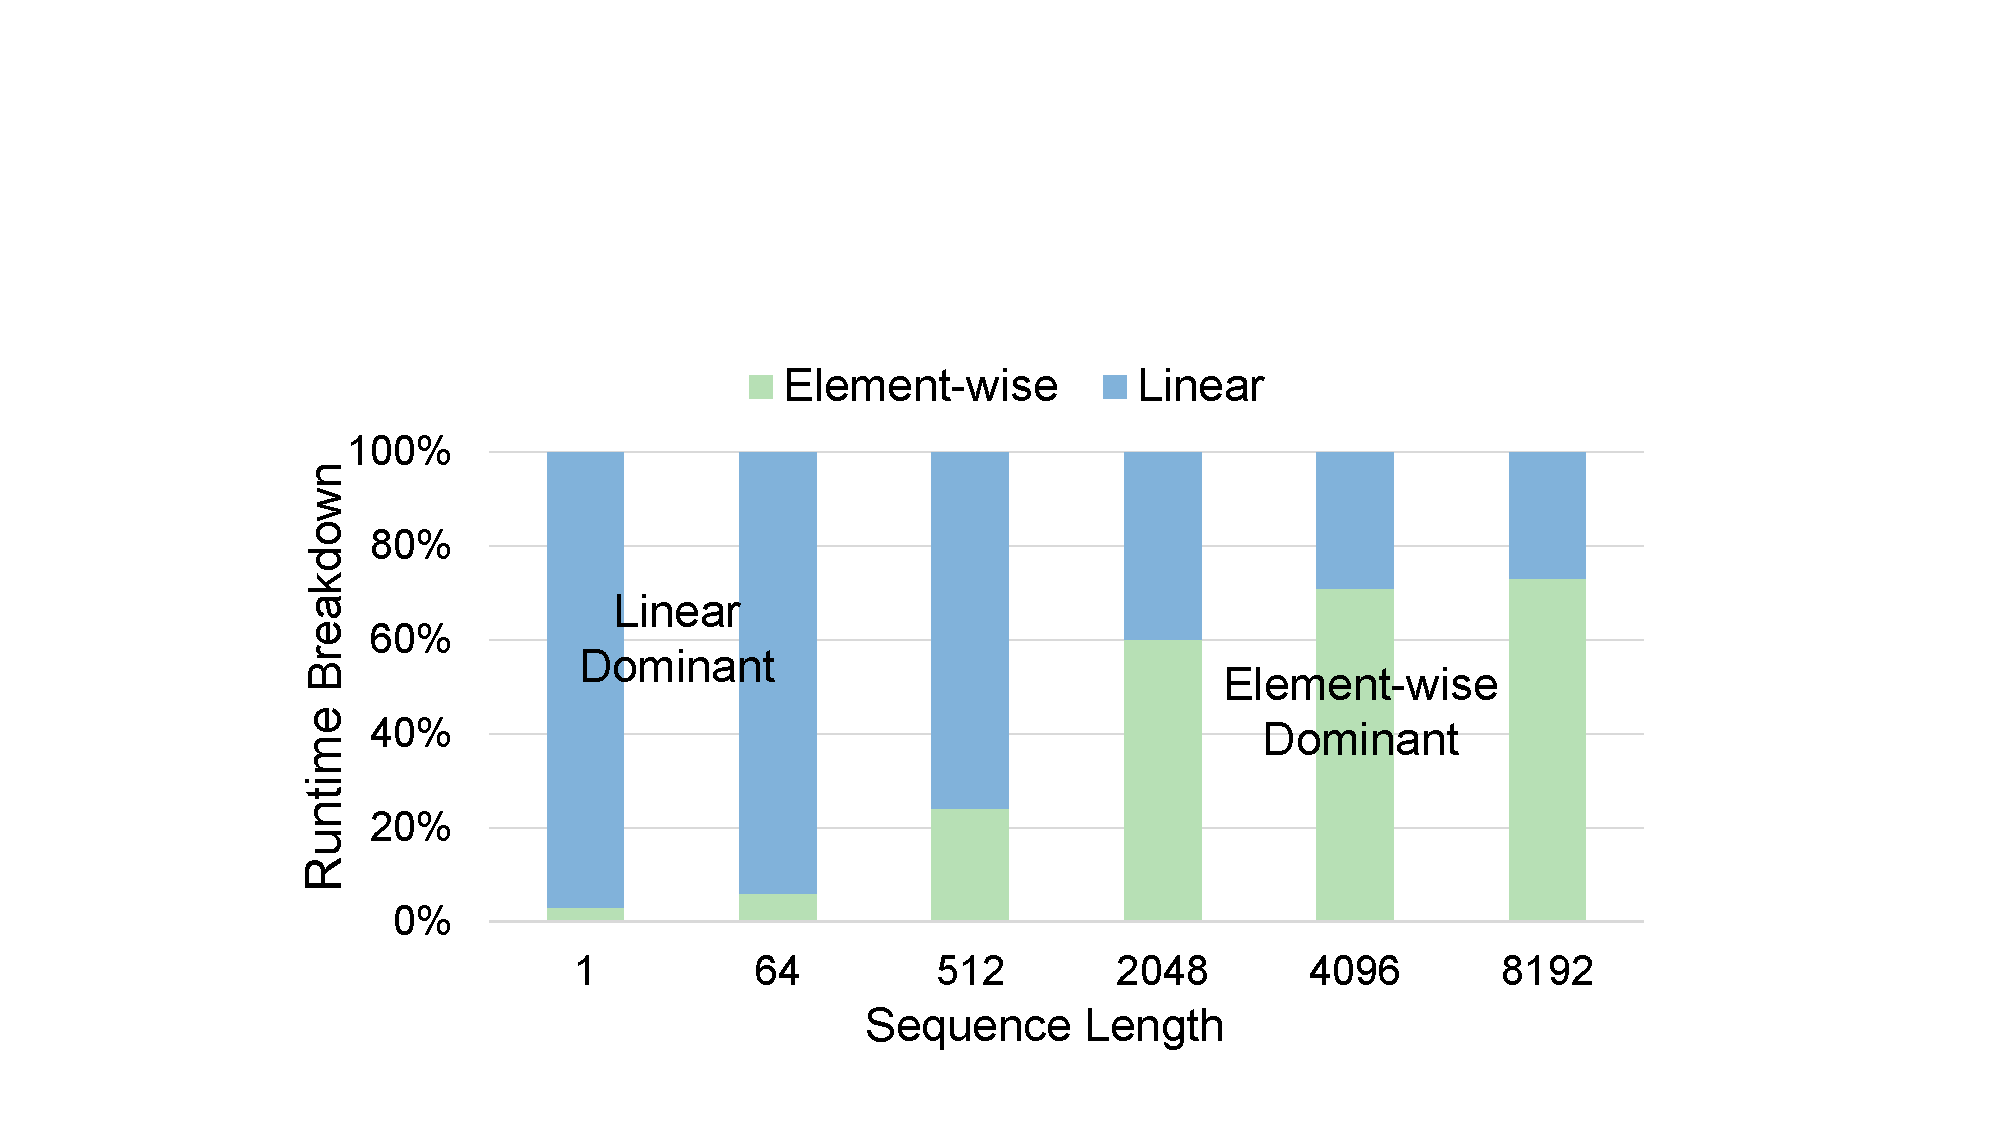
\includegraphics[width=0.4\textwidth]{figures/introduction/breakdown.pdf}
%   \vspace{-12pt}
%   \caption{Runtime breakdown with different sequence lengths in Mamba. Element-wise operations contribute a large fraction of the runtime with long sequence length while linear operations are dominant with short length.}
%   \vspace{-18pt}
%   \label{fig:time_proportion}
% \end{figure}

% %图改成linear用input sharing好，但是element-wise不适用
%  \begin{figure*}[!t]
%   \centering
%   \vspace{-5pt}
%   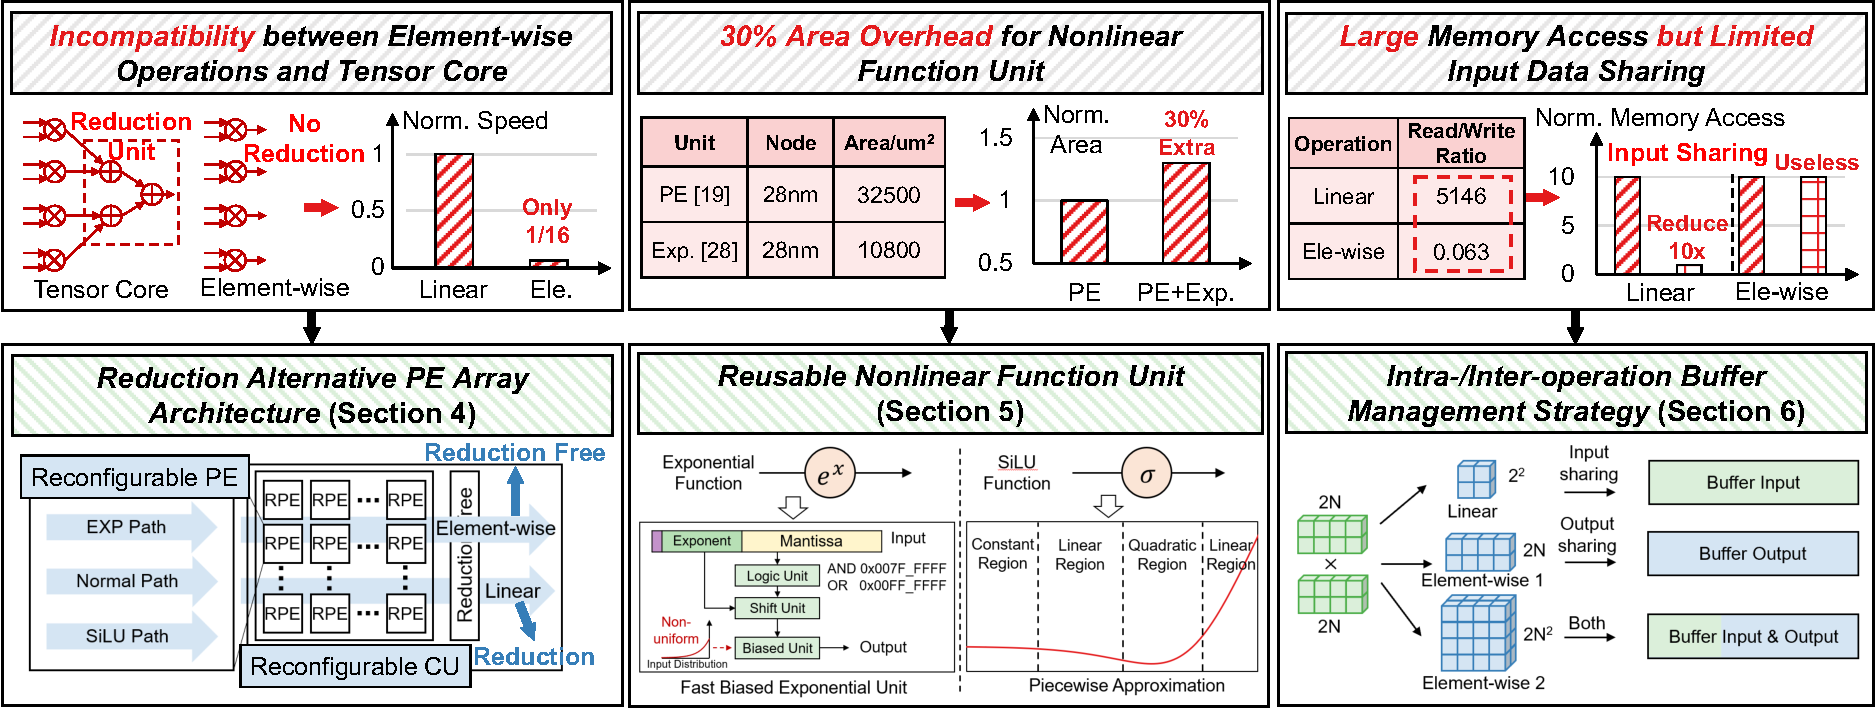
\includegraphics[width=0.98\textwidth]{figures/introduction/overview.pdf}
%   \vspace{-12pt}
%   \caption{Challenges in Mamba computation: (1) incompatibility between element-wise operations and Tensor Core, (2) 30\% area overhead for nonlinear function unit, and (3) large memory access but limited input data sharing for element-wise operations. We propose three novel contributions in \we: (1) reduction alternative PE array architecture, (2) reusable nonlinear function unit, and (3) intra-operation and inter-operation buffer management strategy, to solve these challenges.}
%   \vspace{-15pt}
%   \label{fig:overview}
% \end{figure*}

% However, there is limited research on optimizing for Mamba processing.
% Therefore, we profile the processing carefully and identify three main challenges in Mamba computations:
% \textbf{(1) Incompatibility between element-wise operations and Tensor Core.}
% Linear operations (\textit{e.g.}, matrix multiplication and convolution) and element-wise operations are two dominating operations in Mamba.
% Tensor Core~\cite{tensorcore_a100,tensorcore_h100} is a typical domain specific architecture with reduction tree focused on accelerating these linear operations with high the compute intensity (\textit{e.g.}, $>$1000 FLOPs/Byte).
% However, as shown in Figure~\ref{fig:time_proportion}, the time proportion of element-wise operations escalates significantly as sequence length increases (\textit{e.g.}, $>$60\% with 2048 input length).
% Because the element-wise operations do not need reduction, applying them on Tensor Core-based architecture should introduce large amount of invalid computations, leading to an extreme inefficiency (\textit{e.g.}, 1/16 normalized speed). 
% \textbf{(2) Large area overhead for nonlinear function unit.}
% Exponential function and Sigmoid Linear Unit (SiLU) function are two nonlinear functions in Mamba. Previous methods~\cite{exp_unit,nilsson2014hardware,reggiani2023flex} often design specific unit to compute them, leading to much more area overheads. 
% As shown in Figure~\ref{fig:overview} middle bottom, the optimized nonlinear function unit such exponential function still occupy 30\% of the PE area~\cite{tstc,exp_unit}.
% \textbf{(3) Large memory access but limited input data sharing for element-wise operations.}
% Linear and element-wise operations in Mamba exhibit large compute intensity variance (\textit{e.g.}, $\sim$3 orders of magnitude) and large read/write ratio variance (\textit{e.g.}, $>$3 orders of magnitude). 
% Due to the limited data sharing in element-wise operations, it is useless to apply the existed methods like tiling~\cite{li2019coordinated} to element-wise operations.

% In response to these challenges, we propose \we, a Mamba accelerator with reconfigurable architecture, to support fast and energy-efficient Mamba computations. 
% Our contributions are as follows:
% % \begin{itemize}
%     % \item  
    
% \textbf{(1) Reduction alternative PE array architecture} for both linear and element-wise operations.
% For linear operations, the reduction tree connected to PE arrays is enabled and executes the reduction operation.
% For element-wise operations, the reduction tree is disabled and bypasses the results.
    
% % We propose a reconfigurable architecture controlled by instruction with reconfigurable computing units (RCUs) and processing elements (RPEs). Each RCU is controlled by a reduction tree to support both linear and element-wise operations. Each RPE supports element-wise addition, element-wise multiplication, SiLU, and exponential approximation, to efficiently support both linear and element-wise operations in Mamba.
%     % \item  

% \textbf{(2) Reusable nonlinear function unit} based on reconfigurable PE arrays.
% We decompose the exponential function into element-wise operations and a shift operation by a fast biased exponential algorithm.
%  We also decompose the activation function (SiLU) into a range detection and element-wise operations by a piecewise approximation algorithm.
% Thus, the reconfigurable PEs are fully reused to execute nonlinear functions with negligible accuracy loss.
    
% \textbf{(3) Intra-operation and inter operation buffer management strategy.}
% We propose intra-operation and inter-operation buffer management strategy for linear and element-wise operations. 
% For linear operations, the buffer pool is managed as an input buffer to maximize the input data sharing within each operation. 
% For element-wise operations, the buffer pool is managed as an output buffer to maximize the output data sharing between operations. 
%     % \item  


% % \end{itemize}

% We implement \we in \textit{Verilog} and design a cycle-accurate simulator to evaluate \we. 
% We conduct extensive experiments on Mamba with different model sizes (\textit{i.e.}, Mamba-130M to Mamba-2.8B).
% As a result, \we achieves up to 463.22$\times$/11.66$\times$ speedup and up to 9761.42$\times$/242.52$\times$ energy efficiency compared to Intel Xeon 8358P CPU and NVIDIA Tesla A100 GPU implementations, respectively. 

% %TODO:实验效果
% The rest of this paper is organized as follows. 
% Section~\ref{sec:background} introduces the background of SSM and Mamba model for \we. 
% Three proposed approaches corresponding to the challenges are elaborated in Section~\ref{sec:method1}\textendash\ref{sec:method3}. 
% The overview hardware design of the \we is shown in Section ~\ref{}, and the  . 
% Extensive experimental results are shown in Section~\ref{sec:experiment} and Section~\ref{sec:conclusion} concludes this paper.

%SSM很重要，Mamba的优势，对比transformer，应用场景
%Mamba计算中的问题
%contribution

% \section{Background}\label{sec:background_0329}

\subsection{Detailed Routing Phases}
During routing phases, a large number of design rules need to be processed. 
This process requires determining connection locations for all interconnects while satisfying design constraints at advanced technology nodes, fundamentally representing a path-planning problem with complex constraints in high-dimensional solution space, directly impacting chip performance, power consumption, and manufacturing costs. 
The extreme compression at nanometer scales and exponentially expanding circuit scale have made heuristic routing paradigms relying on iterative optimization particularly challenging, with the intensive computational demands on CPUs emerging as a critical bottleneck constraining both solution quality and optimization efficiency.
To the escalating challenges posed by exponential growth in System-on-Chip (SoC) design complexity under post-Moore's Law paradigms, the open-source EDA flow ''OpenROAD'' has emerged as a cutting-edge solution for complete RTL-to-GDSII implementation. 
Across the design flow, running time is the critical metric and pressing task for IC design automation, especially keeping peace with the quality of the routing resolution. Existing approaches primarily focus on utilizing partition-based multithreaded CPUs to accelerate routing.

In the Physical Design flow, routing is categorized into global routing and detailed routing due to the manufacturability limitations and large time consumption. 
Global routing provides rough guidance with congestion and timing. Detailed routing generates exact rectilinear wiring interconnects based on global routing results, and reduces the design rule violations to satisfy the manufacturability requirements.
Unlike global routing, detailed routing infrastructure is built upon multiple tiers of metal layers. Within each layer, interconnects must be routed along predefined orthogonal tracks oriented either horizontally or vertically. 
Detailed routing is much more time-consuming than global routing due to several factors. 
First, detailed routing must comply with strict design rule constraints (DRC) and conduct multi-dimensional calculations, such as parasitic RC delay modeling and crosstalk analysis. 
Second, the path search space in detailed routing is much larger and more complex, as it operates on fine-grained grids and uses algorithms like maze routing to navigate obstacles. 
Third, detailed routing involves dynamic data management, with high-resolution layout databases requiring frequent DRC checks and incremental static timing analysis. 
Fourth, manufacturing variability necessitates statistical validation and redundancy mechanisms, consuming additional computational resources. 
Finally, toolchain interoperability issues, such as parsing DEF/LEF files and coordination with other modules, introduce significant delays. 
For example, a 7nm design might spend 48 hours on detailed routing compared to 3 hours for global routing.

In ISPD'18[1] and ISPD'19[?] detailed routing contest, detailed routing requires a combination of runtime, and constraints (e.g. minimum-cut, minimum-width, etc.) that have been formed into a better result. This necessitates a holistic consideration of trade-offs between design rule adherence, manufacturability constraints, and multi-objective optimization metrics to balance routing quality with performance targets.
Some excellent detailed routers like TritonRoute [5] and Dr.CU 2.0 [6] come to the fore in the competition. TritonRoute in particular, has been integrated into the OpenROAD open source process and has been adopted by several academic/industrial projects.

Prior research on detailed routing methodologies can be categorized into two complementary dimensions: 
(1) algorithmic advancements for conventional design rule-driven interconnect optimization, 
and (2) hardware-accelerated frameworks leveraging parallel computing architectures to overcome computational bottlenecks inherent in large-scale layout synthesis.

\subsection{Design Rule-Driven Interconnect Optimization}
In the previous work, BonnRoute[2] and RegularRoute[3] have made some breakthroughs in reducing wire lengths/through holes and ensuring design compliance through global resource optimization and rule-based hierarchical routing strategies, respectively. 
Triggered by the ISPD'18 detailed routing contest [1], a multitude of novel routing methodologies have emerged. Kahng et al. [4] partitioned each layer into parallel panels and formulated the routing problem on each panel as an integer linear program. Dr. CU [5] proposed an optimal path searching algorithm handling the minimum-area constraint. 
Based on this, Li et al. proposed DRCU2.0 [6]to improve the routing quality.

The above algorithms have their own innovations in implementation, the core path search mechanism can still be traced back to the classical Maze Routing framework. 
Based on the A* algorithm, modern routers use heuristic functions to guide the search direction, exploring feasible connection paths between source and target layer by layer in the multi-layer routing space. However, 
in the face of increasingly complex metal layer stacks and differentiated design rules, the limitations of traditional single-path search are becoming more and more significant.
For this reason, mainstream advanced routers generally adopt an iterative “Rip-up and Reroute” strategy: 
The first round of wiring tolerates some violations to quickly complete the global connection.
Then the router selectively removes the conflicting wires and re-optimizes their paths by locating the violated areas through Design Rule Check (DRC). 
Although the iterative rip-up and reroute process can progressively improve the \textbf{routing compliance rate}, repeated operations on large-scale nets (\num{1e6} instances) result in,ost of the total runtime being consumed by \textbf{DRC-driven iterative optimization}, establishing it as the dominant efficiency bottleneck in modern detailed routing flows.

\subsection{Hardware Acceleration Framework for Parallel Computing Architecture}
To address the critical challenge of time-consuming routing processes in routing flow, researchers have explored heterogeneous acceleration platforms. 
For path planning acceleration using A* algorithm, Zhou et al.[7] demonstrated 37-75× acceleration via 8-port cache and array-based OPEN lists, but the architecture suffers from inefficient resource utilization when processing high-obstacle-density maps, where frequent cache misses degrade performance predictability. 
Osama et al.[8] developed an FPGA implementation with 50-100× speedup through 8-way parallel evaluators and cache-optimized memory access. Nevertheless, its fixed 256×256 grid mapping and complex 5×5 caching mechanism restrict scalability for large-scale scenarios. 

For maze routing acceleration, Jiang et al.[9] implemented an FPGA-based batched maze routing kernel achieving 3.1× speedup over CPU implementations with <1\% wirelength degradation, but its performance is constrained by data dependency management and limited scalability when handling heterogeneous net sizes. 
Meanwhile, Lin et al.[10] proposed GAMER, a GPU-accelerated maze routing scheme that achieved 16× acceleration for coarsened maze routing through sweeping-style parallelism.
% \todo{}
However, its performance gain diminishes in fine-grained routing stages, and the quality-driven batch partitioning strategy introduces additional scheduling overhead that limits throughput.


%[1] S. Mantik, G. Posser, W.-K. Chow, Y. Ding, and W.-H. Liu, “Ispd 2018 initial detailed routing contest and benchmarks,” in Proceedings of the 2018 International Symposium on Physical Design, ser. ISPD ’p. 140–143,18, 2018.
%[2]M. Gester, D. Müller, T. Nieberg, C. Panten, C. Schulte, and J. Vygen, “BonnRoute: Algorithms and data structures for fast and good VLSI routing,” ACM Trans. Design Automat. Electron. Syst., vol. 18, no. 2, pp. 1–24, 2013.
%[3] Y. Zhang and C. Chu, “RegularRoute: An efficient detailed router applying regular routing patterns,” IEEE Trans. Very Large Scale Integr. (VLSI) Syst., vol. 21, no. 9, pp. 1655–1668, Sep. 2013.
%[4] A. B. Kahng, L. Wang, and B. Xu, “Tritonroute: an initial detailed router for advanced vlsi technologies,” in IEEE/ACM International Conference on Computer-Aided Design (ICCAD), pp. 1–8, IEEE, 2018.
%[5] G. Chen, C.-W. Pui, H. Li, J. Chen, B. Jiang, and E. F. Young, “Detailed routing by sparse grid graph and minimum-area-captured path search,” in IEEE/ACM Asia and South Pacific Design Automation Conference (ASPDAC), pp. 754–760, ACM, 2019.
%[6] H. Li, G. Chen, B. Jiang, J. Chen, and E. F. Y. Young, “Dr. cu 2.0: A scalable detailed routing framework with correct-by-construction design rule satisfaction,” in 2019 IEEE/ACM International Conference on Computer-Aided Design (ICCAD), pp. 1–7,2019.
%[7] Yuzhi Zhou, Xi Jin, Tianqi Wang, "FPGA Implementation of A Algorithm for Real-Time Path Planning", International Journal of Reconfigurable Computing, vol. 2020, pages 11, 2020.
%[8] A. Osama et al., "Fast RTL Implementation of A* Path Planning Algorithm," 2021 International Conference on Microelectronics (ICM), New Cairo City, Egypt, pp. 5-8,2021.
%[9] X. Jiang,Y.Lin, andZ.Wang, “Fpga-accelerated maze routing kernel for vlsi designs,”in Proc. ASPDAC. Virtual Conference:IEEE ,January 2022.
%[10] S. Lin, J. Liu and M. D. F. Wong, "GAMER: GPU Accelerated Maze Routing," 2021 IEEE/ACM International Conference On Computer Aided Design (ICCAD), Munich, Germany,pp. 1-8, 2021

%%%%%%%%
% \section{Background}\label{sec:background}
% \subsection{Preliminaries}
% Routing is the most time-consuming step in the back-end design process.
% Due to its complexity, modern routing is usually divided into global routing and fine-grained routing, while kernel routing algorithms are mostly based on maze routing.
% Among them, as A kind of maze routing, A* is a routing algorithm that is used frequently and has good effect, so it has universal significance to accelerate A*.


% \subsection{Related Works}\label{sec:background:ssm}

% FPGA routing: FPGA routing is essentially an attempt to find disjoint paths on the routing resource graph.
% Shen et al. proposed the first GPU-accelerated FPGA routing using a GPU-friendly single-source Shortest Path (SSSP) kernel.
% Instead of using Dijkstra or A* search algorithms, they used the Bellman-Ford algorithm, which is suitable for massive parallelization on Gpus.
% To increase parallelism, they also restrict search bounding boxes so that networks with bounding boxes that are separate from each other can be routed in parallel.
% In single - and multi-network parallelism, they are 21 times faster than sequential VPR routers.

% ASIC routing: ASIC routing is different from FPGA routing because it works on a grid rather than a graph, and the design rules are more complex.
% Han et al. developed a GPU-accelerated global router and compared it to the high efficiency router NCTUgr 2.0 on CPU.
% By decomposing the multi-pin network into a 2-pin network, as shown in Figure 3, they increase parallelism and simplify routing for each network.
% In the end, they achieved 2.5-3.9 times acceleration and 2.5\% bandwidth attenuation.
% They then improved the network-level concurrent scheduling strategy and GPU implementation maze routing algorithm, achieving a 4.0-fold increase in speed and a 1% decrease in bandwidth compared to another academic router, NTHU-Route 2.0.
% So far, we have not seen any work that can achieve significant acceleration without any loss of quality, because it is very important to make Gpus accelerate even faster than distributed CPU computing.
% At the same time, the acceleration of complex design rules has not been considered in the detailed wiring.

%%%%%%%%%%%%%%
% The continuous state space model in equation~\ref{eq:cont_ssm} defines a linear mapping from an input signal $x(t)\in \mathbb{R}^{M}$ (a function of time $t$) to output signal $y(t)\in \mathbb{R}^{M}$ through a hidden state $h(t) \in \mathbb{R}^{N}$:
% \begin{equation}\label{eq:cont_ssm}
% \begin{split}
%   h'(t) &= A(t)h(t)+B(t)x(t) \\
%    y(t) &= C(t)h(t)
% \end{split}
% \end{equation}
% where state matrix $A(t) \in \mathbb{R}^{N\times N}$, input matrix $B(t) \in \mathbb{R}^{N\times M}$, output matrix $C(t) \in \mathbb{R}^{M\times N}$, and the change of hidden state $h'(t)\in \mathbb{R}^{N}$.
% Classical SSM has dynamic parameters (\textit{e.g.}, $A,B,C$) that change over time. 
% However, when they are constant the dynamics are invariant through time, which is known as a linear time-invariant (LTI) system~\cite{lti}, and is equivalent to a (continuous) convolution.

% Data like words and tokens in the real world is discrete instead of continuous, so equation~\ref{eq:cont_ssm} must be discretized to be applied to an sampled input sequence $x=(x_0,x_1,x_2,...)$ instead of continuous function $x(t)$. 
% An additional step size parameter $\Delta$ is required that represents the resolution of the input. 
% Conceptually, the inputs $x(n)$ can be viewed as uniformly-spaced samples from an implicit underlying continuous signal $x(t)$, where $x(k)=x(k\Delta)$.
% The discretization process from continuous time signal processing to discrete processing is the fact that the SSM has equivalent forms of solving partial differential equations.
% To illustrate discretization, the simplest method is to apply Taylor series method~\cite{taylor} which turns the equation~\ref{eq:cont_ssm} into the first-order approximation:
% \begin{equation}\label{eq:ssm}
% \begin{split}
%   h_n &= h_{n-1}+\Delta(Ah_{n-1}+Bx_{n}) \\
%       &= (I+\Delta A)h_{n-1}+(\Delta B)x_{n} \\
%       &= \overline{A}h_{n-1}+\overline{B}x_n \\
%   y_n &= Ch_n
% \end{split}
% \end{equation}
% where the discrete version of parameters has the same shapes as the original continuous version: $A \in \mathbb{R}^{N\times N}$ and $B \in \mathbb{R}^{N\times M}$. The discretized system depends on $\Delta$ to generate $\Delta A$ and $\Delta B$. 
% Therefore, $\Delta$ can be interpreted as parameters that modulates the SSM instead of as a fixed step size. 

% \begin{figure}[!t]
%   \centering
%   % \vspace{-10pt}
%   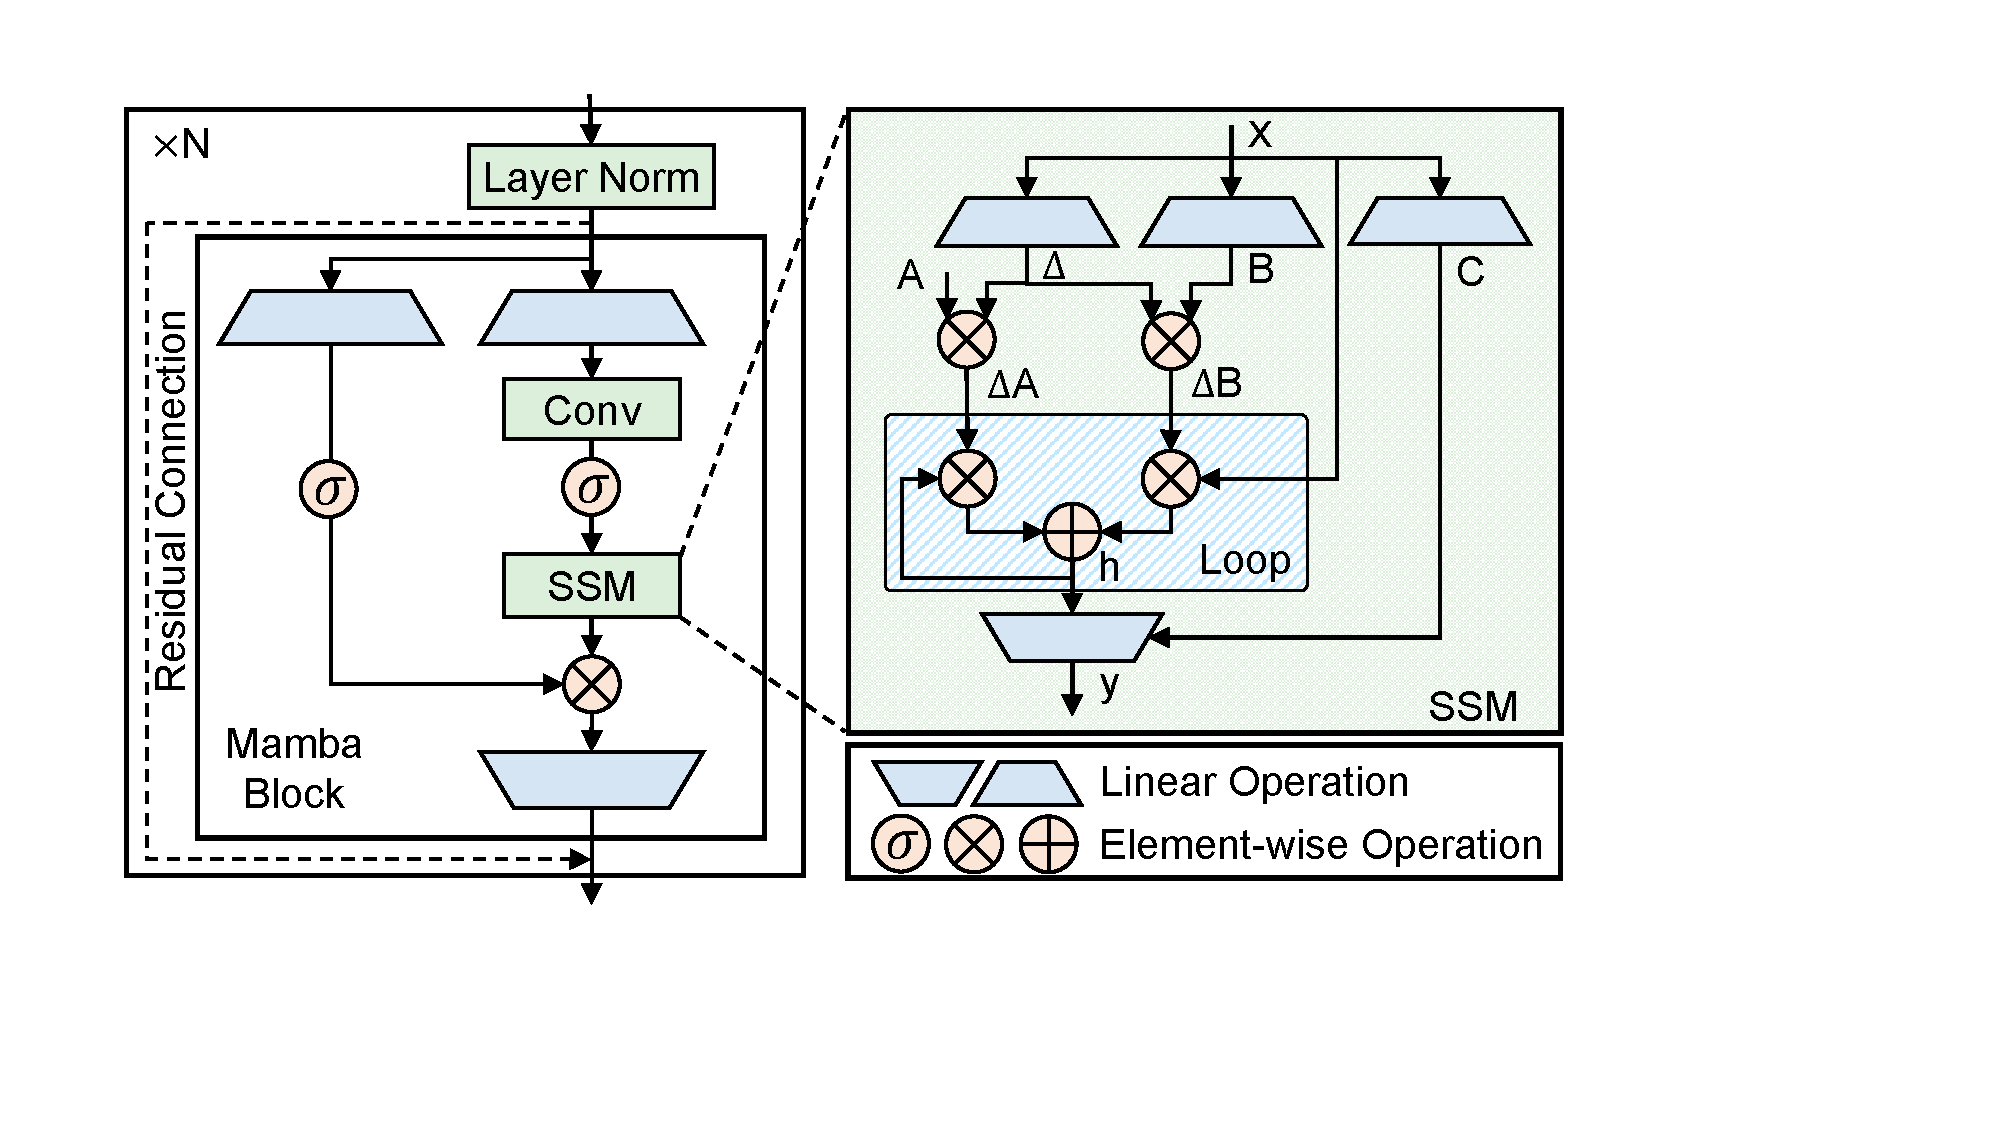
\includegraphics[width=0.47\textwidth]{figures/background/mamba_block.pdf}
%   \vspace{-16pt}
%   \caption{Computational flow in Mamba block and SSM. Mamba model consists of N blocks with residual connection. In SSM, $\Delta$, $B$ and $C$ are generated by input $x$. Then it performs loops to update hidden state $h$, and generates output $y$.}
%   \vspace{-18pt}
%   \label{fig:mamba_block}
% \end{figure}

% \subsection{Mamba}\label{sec:background:mamba}

% Mamba~\cite{mamba} introduces selective mechanism into SSM and proposes an implementation of selective state space model layer.
% Mamba block consists of a layer normalization, several linear projections, a convolution, a SSM block, and a residual connection.
% In each layer, the input sequence is first processed by a linear projection and then processed by the convolution.
% Then it is processed by an activation and then processed by the SSM. 
% After SSM, the main branch is multiplied by the collateral branch including a linear projection and an activation (\textit{e.g.}, SiLU~\cite{silu}) to generate the combined result.
% After combination, the result is processed by a linear projection.
% Last, the result is added back to the input through the residual connection~\cite{resnet}. 
% Instead of interleaving Mamba block and Feed-forward block, Mamba simply repeats the Mamba block homogenously. 

% During SSM processing, the input $x$ undergoes a series of transformations. 
% Firstly, it is subjected to three linear projections, resulting in $\Delta$, $B$ and $C$. 
% Subsequently, $\Delta$ is involved in the Einstein summation operations~\cite{einsum} with $A$ and $B$ separately, generating $\Delta A$ and $\Delta B$. 
% These intermediate results $\Delta A$ and $\Delta B$ are then multiplied with the hidden state and input $x$ by element-wise Einstein summation, respectively. 
% After $L$ (sequence length) times iterations, the hidden state is updated for $L$ times. 
% The outcomes of these operations are then combined through addition, resulting in the updated hidden state. 
% Finally, the updated hidden state undergoes matrix multiplication with $C$, followed by a linear transformation, to generate the output. The whole computational flow in Mamba block is illustrated in Figure \ref{fig:mamba_block}.



% \subsection{Tensor Core}\label{sec:background:tc}




\section{Background}\label{sec:background_0329}

\subsection{Detailed Routing Phases}
During routing phases, a large number of design rules need to be processed. 
This process requires determining connection locations for all interconnects while satisfying design constraints at advanced technology nodes, fundamentally representing a path-planning problem with complex constraints in high-dimensional solution space, directly impacting chip performance, power consumption, and manufacturing costs. 
The extreme compression at nanometer scales and exponentially expanding circuit scale have made heuristic routing paradigms relying on iterative optimization particularly challenging, with the intensive computational demands on CPUs emerging as a critical bottleneck constraining both solution quality and optimization efficiency.
To the escalating challenges posed by exponential growth in System-on-Chip (SoC) design complexity under post-Moore's Law paradigms, the open-source EDA flow ''OpenROAD'' has emerged as a cutting-edge solution for complete RTL-to-GDSII implementation. 
Across the design flow, running time is the critical metric and pressing task for IC design automation, especially keeping peace with the quality of the routing resolution. Existing approaches primarily focus on utilizing partition-based multithreaded CPUs to accelerate routing.

In the Physical Design flow, routing is categorized into global routing and detailed routing due to the manufacturability limitations and large time consumption. 
Global routing provides rough guidance with congestion and timing. Detailed routing generates exact rectilinear wiring interconnects based on global routing results, and reduces the design rule violations to satisfy the manufacturability requirements.
Unlike global routing, detailed routing infrastructure is built upon multiple tiers of metal layers. Within each layer, interconnects must be routed along predefined orthogonal tracks oriented either horizontally or vertically. 
Detailed routing is much more time-consuming than global routing due to several factors. 
First, detailed routing must comply with strict design rule constraints (DRC) and conduct multi-dimensional calculations, such as parasitic RC delay modeling and crosstalk analysis. 
Second, the path search space in detailed routing is much larger and more complex, as it operates on fine-grained grids and uses algorithms like maze routing to navigate obstacles. 
Third, detailed routing involves dynamic data management, with high-resolution layout databases requiring frequent DRC checks and incremental static timing analysis. 
Fourth, manufacturing variability necessitates statistical validation and redundancy mechanisms, consuming additional computational resources. 
Finally, toolchain interoperability issues, such as parsing DEF/LEF files and coordination with other modules, introduce significant delays. 
For example, a 7nm design might spend 48 hours on detailed routing compared to 3 hours for global routing.

In ISPD'18[1] and ISPD'19[?] detailed routing contest, detailed routing requires a combination of runtime, and constraints (e.g. minimum-cut, minimum-width, etc.) that have been formed into a better result. This necessitates a holistic consideration of trade-offs between design rule adherence, manufacturability constraints, and multi-objective optimization metrics to balance routing quality with performance targets.
Some excellent detailed routers like TritonRoute [5] and Dr.CU 2.0 [6] come to the fore in the competition. TritonRoute in particular, has been integrated into the OpenROAD open source process and has been adopted by several academic/industrial projects.

Prior research on detailed routing methodologies can be categorized into two complementary dimensions: 
(1) algorithmic advancements for conventional design rule-driven interconnect optimization, 
and (2) hardware-accelerated frameworks leveraging parallel computing architectures to overcome computational bottlenecks inherent in large-scale layout synthesis.

% \subsection{Design Rule-Driven Interconnect Optimization}
% In the previous work, BonnRoute[2] and RegularRoute[3] have made some breakthroughs in reducing wire lengths/through holes and ensuring design compliance through global resource optimization and rule-based hierarchical routing strategies, respectively. 
% Triggered by the ISPD'18 detailed routing contest [1], a multitude of novel routing methodologies have emerged. Kahng et al. [4] partitioned each layer into parallel panels and formulated the routing problem on each panel as an integer linear program. Dr. CU [5] proposed an optimal path searching algorithm handling the minimum-area constraint. 
% Based on this, Li et al. proposed DRCU2.0 [6]to improve the routing quality.

% The above algorithms have their own innovations in implementation, the core path search mechanism can still be traced back to the classical Maze Routing framework. 
% Based on the A* algorithm, modern routers use heuristic functions to guide the search direction, exploring feasible connection paths between source and target layer by layer in the multi-layer routing space. However, 
% in the face of increasingly complex metal layer stacks and differentiated design rules, the limitations of traditional single-path search are becoming more and more significant.
% For this reason, mainstream advanced routers generally adopt an iterative “Rip-up and Reroute” strategy: 
% The first round of wiring tolerates some violations to quickly complete the global connection.
% Then the router selectively removes the conflicting wires and re-optimizes their paths by locating the violated areas through Design Rule Check (DRC). 
% Although the iterative rip-up and reroute process can progressively improve the \textbf{routing compliance rate}, repeated operations on large-scale nets (\num{1e6} instances) result in,ost of the total runtime being consumed by \textbf{DRC-driven iterative optimization}, establishing it as the dominant efficiency bottleneck in modern detailed routing flows.

% \subsection{Hardware Acceleration Framework for Parallel Computing Architecture}
%To address the critical challenge of time-consuming routing processes in routing flow, researchers have explored heterogeneous acceleration platforms. 
%For path planning acceleration using A* algorithm, Zhou et al.[7] demonstrated 37-75× acceleration via 8-port cache and array-based OPEN lists, but the architecture suffers from inefficient resource utilization when processing high-obstacle-density maps, where frequent cache misses degrade performance predictability. 
%Osama et al.[8] developed an FPGA implementation with 50-100× speedup through 8-way parallel evaluators and cache-optimized memory access. Nevertheless, its fixed 256×256 grid mapping and complex 5×5 caching mechanism restrict scalability for large-scale scenarios. 

%For maze routing acceleration, Jiang et al.[9] implemented an FPGA-based batched maze routing kernel achieving 3.1× speedup over CPU implementations with <1\% wirelength degradation, but its performance is constrained by data dependency management and limited scalability when handling heterogeneous net sizes. 
%Meanwhile, Lin et al.[10] proposed GAMER, a GPU-accelerated maze routing scheme that achieved 16× acceleration for coarsened maze routing through sweeping-style parallelism.
% \todo{}
%However, its performance gain diminishes in fine-grained routing stages, and the quality-driven batch partitioning strategy introduces additional scheduling overhead that limits throughput.


%[1] S. Mantik, G. Posser, W.-K. Chow, Y. Ding, and W.-H. Liu, “Ispd 2018 initial detailed routing contest and benchmarks,” in Proceedings of the 2018 International Symposium on Physical Design, ser. ISPD ’p. 140–143,18, 2018.
%[2]M. Gester, D. Müller, T. Nieberg, C. Panten, C. Schulte, and J. Vygen, “BonnRoute: Algorithms and data structures for fast and good VLSI routing,” ACM Trans. Design Automat. Electron. Syst., vol. 18, no. 2, pp. 1–24, 2013.
%[3] Y. Zhang and C. Chu, “RegularRoute: An efficient detailed router applying regular routing patterns,” IEEE Trans. Very Large Scale Integr. (VLSI) Syst., vol. 21, no. 9, pp. 1655–1668, Sep. 2013.
%[4] A. B. Kahng, L. Wang, and B. Xu, “Tritonroute: an initial detailed router for advanced vlsi technologies,” in IEEE/ACM International Conference on Computer-Aided Design (ICCAD), pp. 1–8, IEEE, 2018.
%[5] G. Chen, C.-W. Pui, H. Li, J. Chen, B. Jiang, and E. F. Young, “Detailed routing by sparse grid graph and minimum-area-captured path search,” in IEEE/ACM Asia and South Pacific Design Automation Conference (ASPDAC), pp. 754–760, ACM, 2019.
%[6] H. Li, G. Chen, B. Jiang, J. Chen, and E. F. Y. Young, “Dr. cu 2.0: A scalable detailed routing framework with correct-by-construction design rule satisfaction,” in 2019 IEEE/ACM International Conference on Computer-Aided Design (ICCAD), pp. 1–7,2019.
%[7] Yuzhi Zhou, Xi Jin, Tianqi Wang, "FPGA Implementation of A Algorithm for Real-Time Path Planning", International Journal of Reconfigurable Computing, vol. 2020, pages 11, 2020.
%[8] A. Osama et al., "Fast RTL Implementation of A* Path Planning Algorithm," 2021 International Conference on Microelectronics (ICM), New Cairo City, Egypt, pp. 5-8,2021.
%[9] X. Jiang,Y.Lin, andZ.Wang, “Fpga-accelerated maze routing kernel for vlsi designs,”in Proc. ASPDAC. Virtual Conference:IEEE ,January 2022.
%[10] S. Lin, J. Liu and M. D. F. Wong, "GAMER: GPU Accelerated Maze Routing," 2021 IEEE/ACM International Conference On Computer Aided Design (ICCAD), Munich, Germany,pp. 1-8, 2021

%%%%%%%%
% \section{Background}\label{sec:background}
% \subsection{Preliminaries}
% Routing is the most time-consuming step in the back-end design process.
% Due to its complexity, modern routing is usually divided into global routing and fine-grained routing, while kernel routing algorithms are mostly based on maze routing.
% Among them, as A kind of maze routing, A* is a routing algorithm that is used frequently and has good effect, so it has universal significance to accelerate A*.


% \subsection{Related Works}\label{sec:background:ssm}

% FPGA routing: FPGA routing is essentially an attempt to find disjoint paths on the routing resource graph.
% Shen et al. proposed the first GPU-accelerated FPGA routing using a GPU-friendly single-source Shortest Path (SSSP) kernel.
% Instead of using Dijkstra or A* search algorithms, they used the Bellman-Ford algorithm, which is suitable for massive parallelization on Gpus.
% To increase parallelism, they also restrict search bounding boxes so that networks with bounding boxes that are separate from each other can be routed in parallel.
% In single - and multi-network parallelism, they are 21 times faster than sequential VPR routers.

% ASIC routing: ASIC routing is different from FPGA routing because it works on a grid rather than a graph, and the design rules are more complex.
% Han et al. developed a GPU-accelerated global router and compared it to the high efficiency router NCTUgr 2.0 on CPU.
% By decomposing the multi-pin network into a 2-pin network, as shown in Figure 3, they increase parallelism and simplify routing for each network.
% In the end, they achieved 2.5-3.9 times acceleration and 2.5\% bandwidth attenuation.
% They then improved the network-level concurrent scheduling strategy and GPU implementation maze routing algorithm, achieving a 4.0-fold increase in speed and a 1% decrease in bandwidth compared to another academic router, NTHU-Route 2.0.
% So far, we have not seen any work that can achieve significant acceleration without any loss of quality, because it is very important to make Gpus accelerate even faster than distributed CPU computing.
% At the same time, the acceleration of complex design rules has not been considered in the detailed wiring.

%%%%%%%%%%%%%%
% The continuous state space model in equation~\ref{eq:cont_ssm} defines a linear mapping from an input signal $x(t)\in \mathbb{R}^{M}$ (a function of time $t$) to output signal $y(t)\in \mathbb{R}^{M}$ through a hidden state $h(t) \in \mathbb{R}^{N}$:
% \begin{equation}\label{eq:cont_ssm}
% \begin{split}
%   h'(t) &= A(t)h(t)+B(t)x(t) \\
%    y(t) &= C(t)h(t)
% \end{split}
% \end{equation}
% where state matrix $A(t) \in \mathbb{R}^{N\times N}$, input matrix $B(t) \in \mathbb{R}^{N\times M}$, output matrix $C(t) \in \mathbb{R}^{M\times N}$, and the change of hidden state $h'(t)\in \mathbb{R}^{N}$.
% Classical SSM has dynamic parameters (\textit{e.g.}, $A,B,C$) that change over time. 
% However, when they are constant the dynamics are invariant through time, which is known as a linear time-invariant (LTI) system~\cite{lti}, and is equivalent to a (continuous) convolution.

% Data like words and tokens in the real world is discrete instead of continuous, so equation~\ref{eq:cont_ssm} must be discretized to be applied to an sampled input sequence $x=(x_0,x_1,x_2,...)$ instead of continuous function $x(t)$. 
% An additional step size parameter $\Delta$ is required that represents the resolution of the input. 
% Conceptually, the inputs $x(n)$ can be viewed as uniformly-spaced samples from an implicit underlying continuous signal $x(t)$, where $x(k)=x(k\Delta)$.
% The discretization process from continuous time signal processing to discrete processing is the fact that the SSM has equivalent forms of solving partial differential equations.
% To illustrate discretization, the simplest method is to apply Taylor series method~\cite{taylor} which turns the equation~\ref{eq:cont_ssm} into the first-order approximation:
% \begin{equation}\label{eq:ssm}
% \begin{split}
%   h_n &= h_{n-1}+\Delta(Ah_{n-1}+Bx_{n}) \\
%       &= (I+\Delta A)h_{n-1}+(\Delta B)x_{n} \\
%       &= \overline{A}h_{n-1}+\overline{B}x_n \\
%   y_n &= Ch_n
% \end{split}
% \end{equation}
% where the discrete version of parameters has the same shapes as the original continuous version: $A \in \mathbb{R}^{N\times N}$ and $B \in \mathbb{R}^{N\times M}$. The discretized system depends on $\Delta$ to generate $\Delta A$ and $\Delta B$. 
% Therefore, $\Delta$ can be interpreted as parameters that modulates the SSM instead of as a fixed step size. 

% \begin{figure}[!t]
%   \centering
%   % \vspace{-10pt}
%   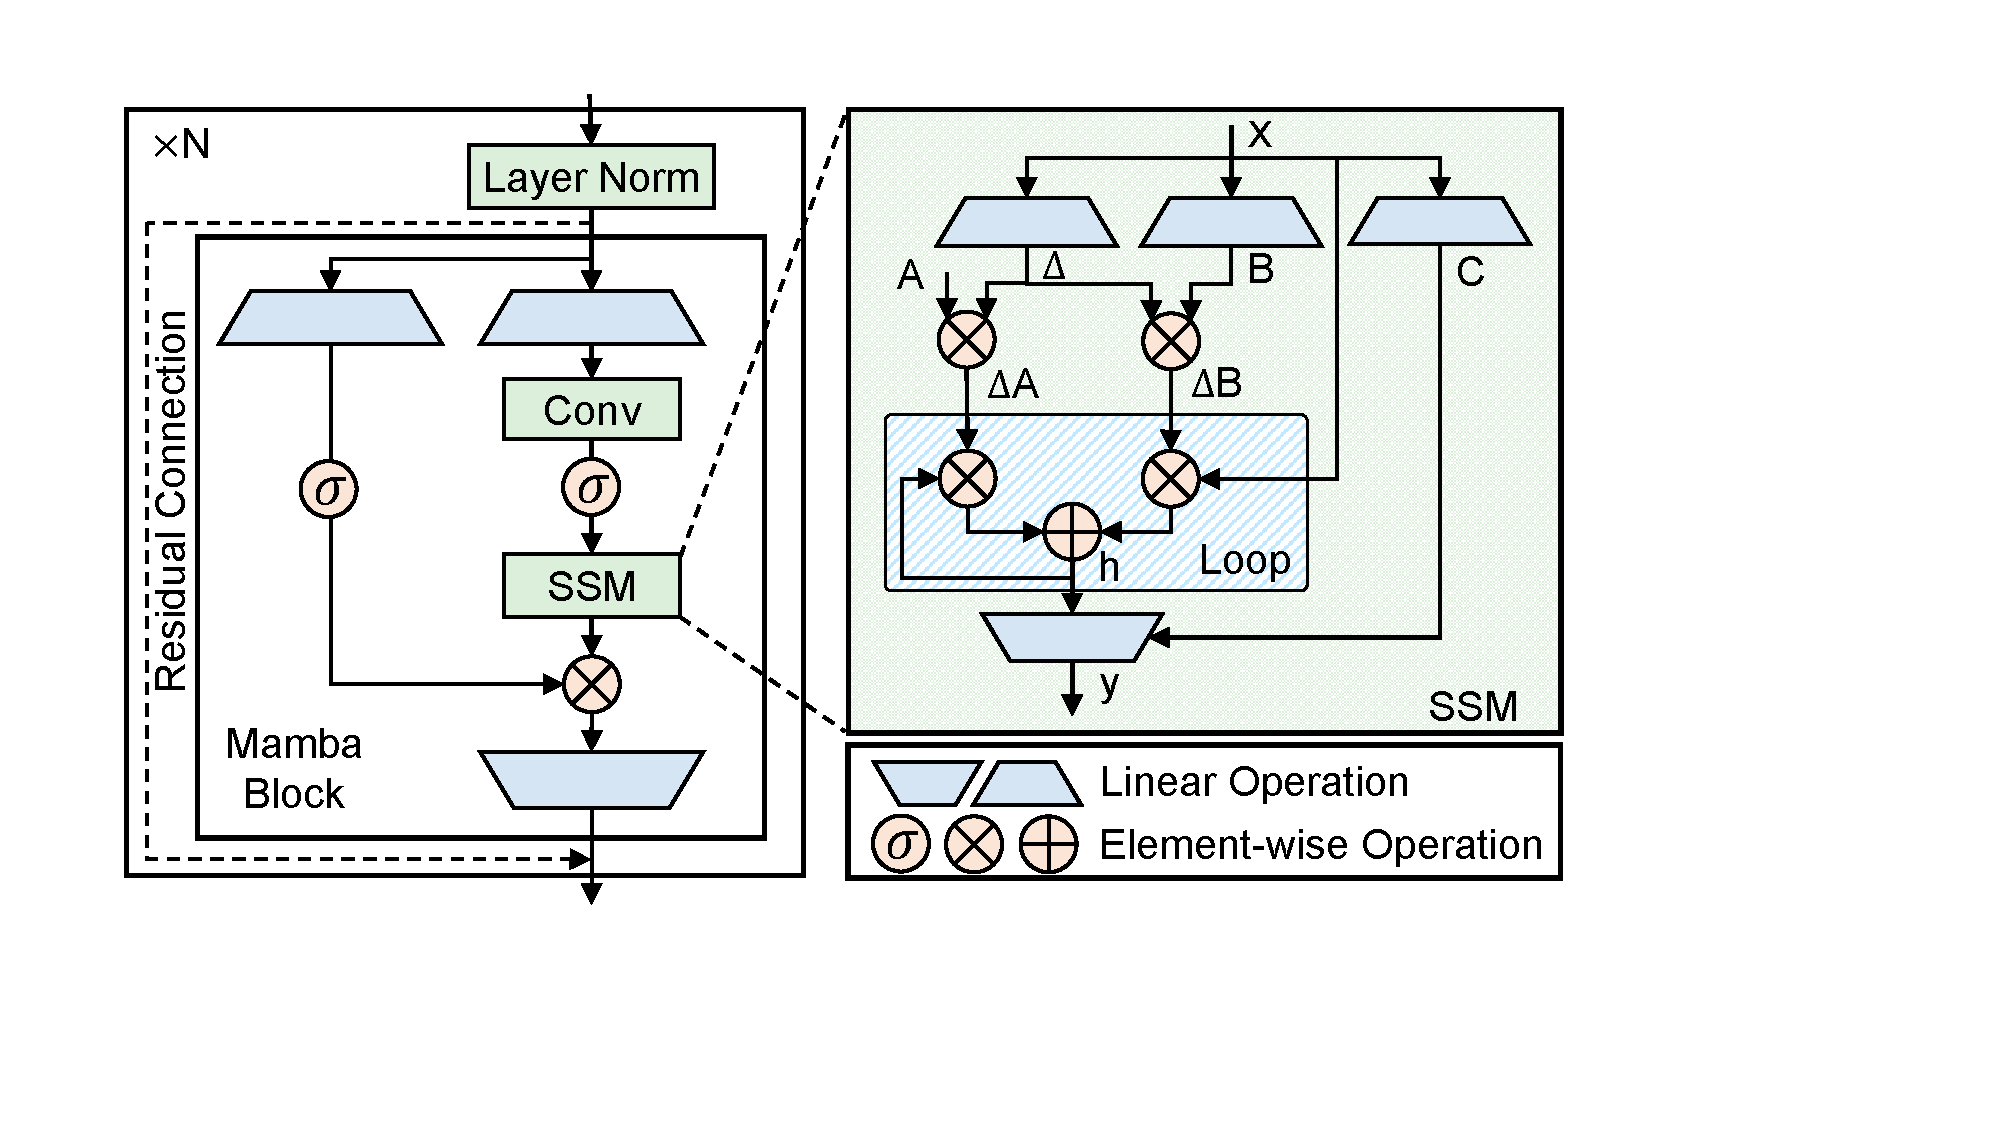
\includegraphics[width=0.47\textwidth]{figures/background/mamba_block.pdf}
%   \vspace{-16pt}
%   \caption{Computational flow in Mamba block and SSM. Mamba model consists of N blocks with residual connection. In SSM, $\Delta$, $B$ and $C$ are generated by input $x$. Then it performs loops to update hidden state $h$, and generates output $y$.}
%   \vspace{-18pt}
%   \label{fig:mamba_block}
% \end{figure}

% \subsection{Mamba}\label{sec:background:mamba}

% Mamba~\cite{mamba} introduces selective mechanism into SSM and proposes an implementation of selective state space model layer.
% Mamba block consists of a layer normalization, several linear projections, a convolution, a SSM block, and a residual connection.
% In each layer, the input sequence is first processed by a linear projection and then processed by the convolution.
% Then it is processed by an activation and then processed by the SSM. 
% After SSM, the main branch is multiplied by the collateral branch including a linear projection and an activation (\textit{e.g.}, SiLU~\cite{silu}) to generate the combined result.
% After combination, the result is processed by a linear projection.
% Last, the result is added back to the input through the residual connection~\cite{resnet}. 
% Instead of interleaving Mamba block and Feed-forward block, Mamba simply repeats the Mamba block homogenously. 

% During SSM processing, the input $x$ undergoes a series of transformations. 
% Firstly, it is subjected to three linear projections, resulting in $\Delta$, $B$ and $C$. 
% Subsequently, $\Delta$ is involved in the Einstein summation operations~\cite{einsum} with $A$ and $B$ separately, generating $\Delta A$ and $\Delta B$. 
% These intermediate results $\Delta A$ and $\Delta B$ are then multiplied with the hidden state and input $x$ by element-wise Einstein summation, respectively. 
% After $L$ (sequence length) times iterations, the hidden state is updated for $L$ times. 
% The outcomes of these operations are then combined through addition, resulting in the updated hidden state. 
% Finally, the updated hidden state undergoes matrix multiplication with $C$, followed by a linear transformation, to generate the output. The whole computational flow in Mamba block is illustrated in Figure \ref{fig:mamba_block}.



% \subsection{Tensor Core}\label{sec:background:tc}


\subsection{Memory Access Bottleneck}
The core of routing algorithms lies in the highly efficient heuristic path-planning method, like the A-star (or A$\ast$ ) search algorithm.  
However, the existing optimizations on the A* algorithm are mainly aimed at computational optimization, and the bottleneck in 
maintaining the open list and a closed list is obviously outstanding, especially when performing many iterative operations.  
For the typical path planning method (A*)acceleration by using FPGA, Zhou et al.[7] demonstrated 37-751$\times$ acceleration via 8-port cache 
and array-based OPEN lists, but the architecture suffers from inefficient resource utilization when processing high-obstacle density maps,
where frequent cache misses degrade performance predictability. 

Osama et al.[8] developed an FPGA implementation with 50-1001$\times$ speedup through 8-way parallel evaluators and cache-optimized memory access. 
Nevertheless, its fixed 256$\times$256 grid mapping and complex 5$\times$5 caching mechanism restrict scalability for large-scale scenarios. 
Jiang et al.[9] implemented an FPGA-based batched maze routing kernel achieving 3.11$\times$ speedup over CPU implementations with < 1\% 
wirelength degradation, but its performance is constrained by data dependency management and limited scalability when handling heterogeneous net sizes. 
Meanwhile, Lin et al.[10] proposed GAMER, a GPU-accelerated maze routing scheme that achieved 161$\times$ acceleration for coarsened maze routing through sweeping-style parallelism. 
However, its performance gain diminishes in fine-grained routing stages, and the qualitydriven batch partitioning strategy introduces 
additional scheduling overhead that limits throughput. 

\begin{figure}[htbp]
    \centering
    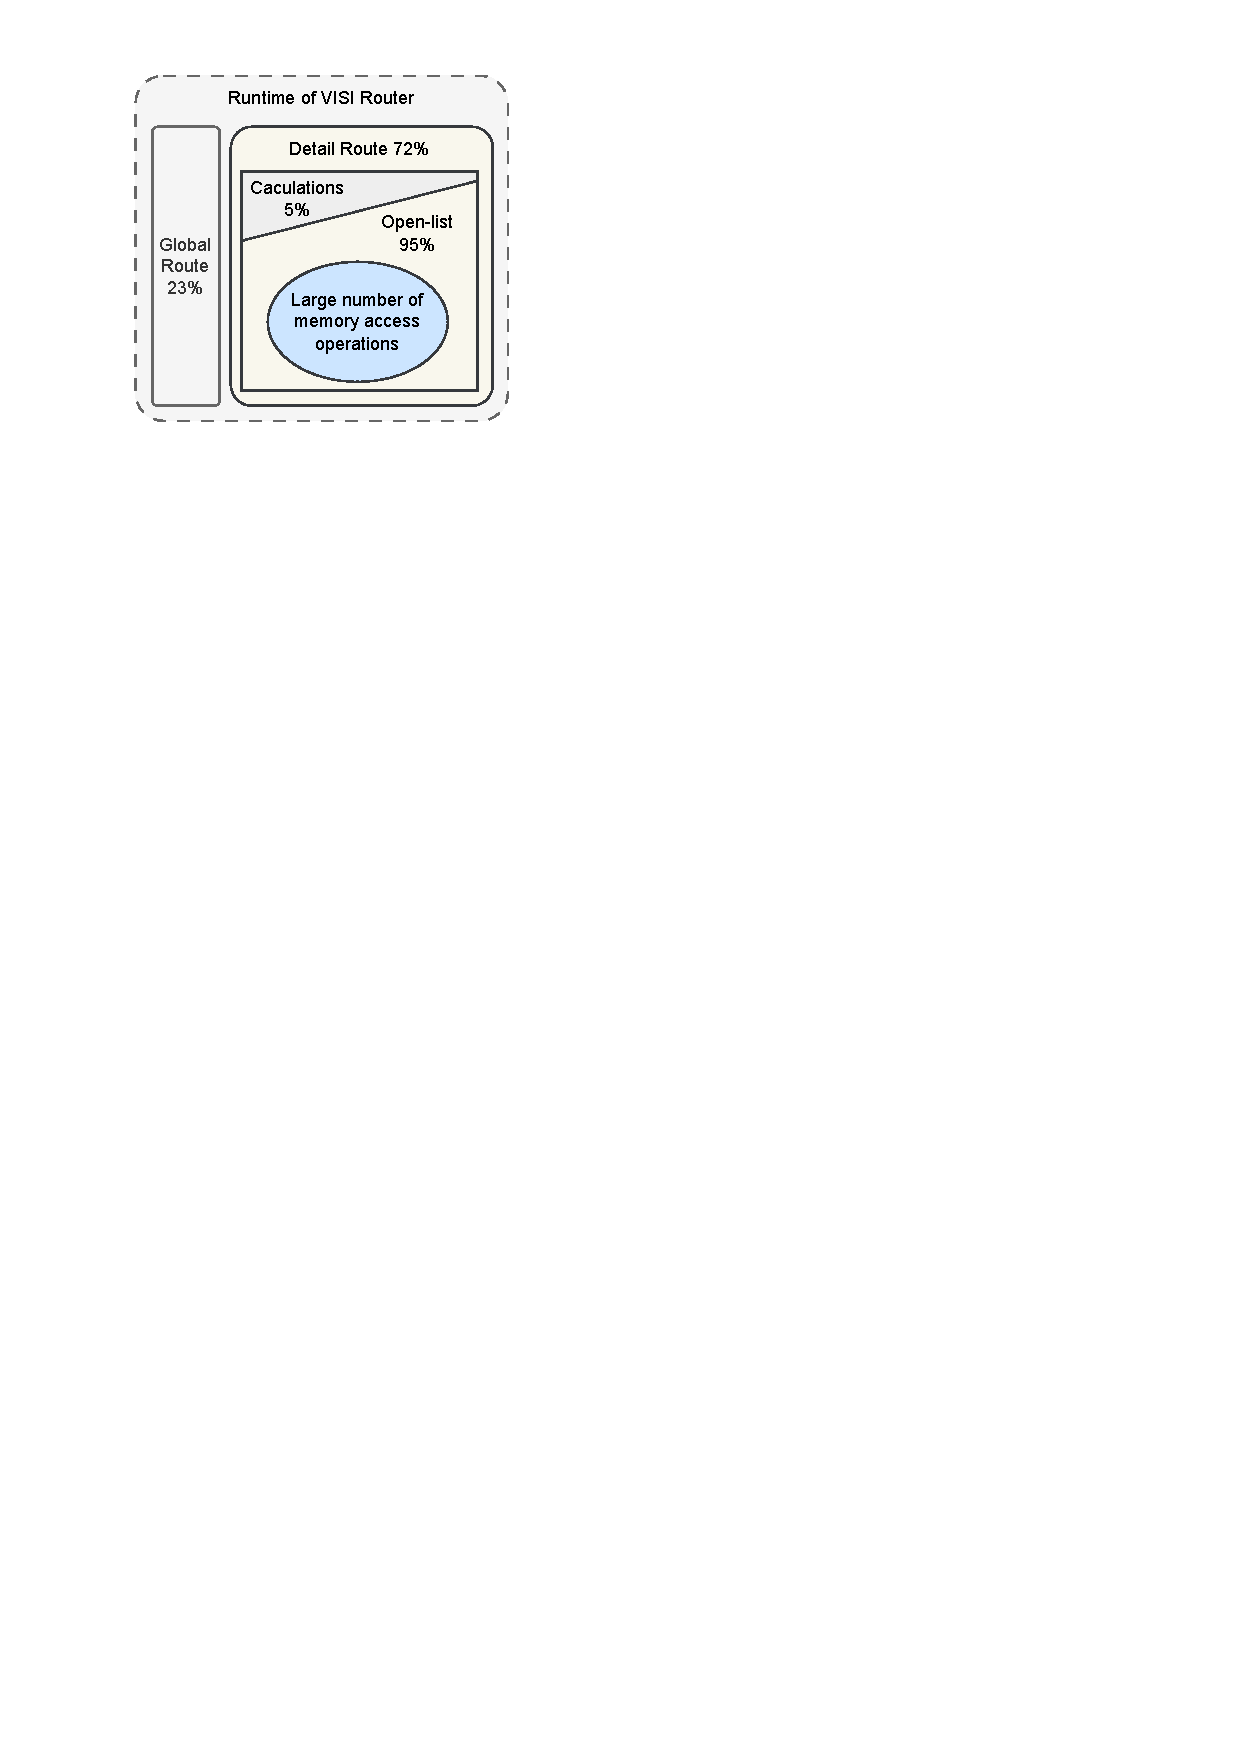
\includegraphics[width=7cm]{figures/background/Execution Time.pdf}
    \caption{Detailed routing takes up most time in the routing process, and most of it is memory access time.}
    \label{fig:Execution Time} % 标签紧跟标题
\end{figure}

\subsection{Versatility and Scalability}
The above proposed acceleration methodology for detailed routing preserves the quality of the entire implementation flow for 
multithreaded FPGA core architectures. Actually, the accelerated A* techniques exhibit broad applicability across various path-searching 
implementations. Given the fundamental similarities in routing paradigms,  particularly in maze routing algorithms and heuristic flow implementation 
methodologies, these acceleration strategies demonstrate significant transfer potential beyond the specific use cases examined in this study. 

\section{Algorthm}
\subsection{Detailed Routing Algorthm Analysis}

Conventional framework of detailed routing algorithm we employ follows a structured flow, as illustrated in Algorithm 1. 
Given the global routing results of the benchmarks (e.g..def and.guides files), we perform a track assignment step following the method described in [11], aligning all nets to predefined routing tracks. 
This preprocessing phase extracts and constructs essential data structures, such as routing grids, net objects, and guide constraints, which serve as inputs to the detailed routing engine. 
The ultimate goal is to produce a DRC-clean routing result with full connectivity, starting from these coarse global routing guides.

%%eg [11]M.-P. Wong, W.-H. Liu, and T.-C. Wang, “Negotiation-based track assignment considering local nets,” in Proc. 21st Asia South Pac. Design Automat. Conf. (ASP-DAC), Macau, China, 2016, pp. 378–383.

\begin{algorithm}[hpt]
\caption{Detailed Routing Flow}
\label{alg:detail_routing_algorithm}
\begin{algorithmic}[1]
\Statex \textbf{Input:} base-data structure, global routing guides
\Statex \textbf{Output:} full connected nets
\STATE \text{InitDb()}, \text{InitPreRouteNet()}

\WHILE{$iter < maxIter$}
    \STATE \text {$drcNets \gets [net_{i}: while$ $ net_{i} \in Nets,$$if$ $net_{i}.drcScore \neq 0]$}
    \WHILE{$\text{$net$} \in \text{$drcNets$}$}
        \STATE $\text{$ucPins$} \gets \text{$GetPins(net)$}$
        \WHILE {$ucPins \neq \emptyset$}
            \STATE $\text{$tpin$} \gets \mathop{\arg\max}\limits_{pin \in ucPins} \text{$pin.cost$}$
            \STATE $\text{$cPins$} \gets \text{$cPins$} \cup \text{$tPin$}$, $\text{$ucPins$} \gets \text{$ucPins$} \setminus \text{$tPin$}$
            \STATE $\text{$sPin$} \gets \text{GetNextPin(\text{$ucPins$})}$
            \STATE \text{FPGA-OptimizedRoutingKernel($sPin$,$cPins$)}
        \ENDWHILE
    \ENDWHILE
    
    \STATE \text{UpdateDRC()}, \text{UpdateNets()}
\ENDWHILE
\STATE \text{UpdateDb()}
\end{algorithmic}
\end{algorithm}


The detailed routing flow, as depicted in Algorithm 1, comprises multiple sequential phases. Initially, the design database is initialized via InitDb(), and essential nets are pre-routed using InitPreRouteNet(). Following this, nets are evaluated based on their design rule check scores, and those exhibiting violations are prioritized for further processing.
The outer loop (lines 2 to 14) performs iterative rip-up and reroute operations, bounded by a predefined maximum iteration count. In each iteration, the set of nets with non-zero DRC scores is extracted. For each net in drcNets, the set of unconnected pins is identified (line 5). The algorithm proceeds to incrementally connect these pins by repeatedly selecting the pin with the highest routing cost as the current target, moving it to the connected pin set, and identifying the next nearest source pin (lines 6–9).
Routing between the selected source and target pins uses the Optimized Routing kernel, which leverages high-throughput hardware acceleration. This process continues until all pins in the net are connected. After net-level rerouting, the global DRC state and net data structures are updated accordingly . Upon convergence or exhaustion of iterations, a final database update is performed, reflecting the complete routing solution.


\subsection{Routing Kernel and Generating Routing Graphs Algorthm Analysis}
The most popular detailed routing methods, like TritonRoute[?] and Dr. CU[?], are both executed by the maze routing kernel to connect all pins on the nets with minimal cost. 
In the actual computing stage, the nets will first abstracted as grid graphs. Each pin pn is equivalent to a set of vertices Sn located on its position, 
then utilize the priority queue and some heuristic methods to improve the quality and speed.Taking TritonRoute[?] as an example, it uses A* (A-STAR) algorithm to explore the route and sets weight for each node.
The weight is a heuristic function f (x) : f (x) = g(x) + h(x), where the function g(x) is the distance or cost from the starting node to current state x, and the function h(x) defines the estimated distance or cost from current state x to the end node. 
We call the function value of f (x) the f value. 


\begin{algorithm}[hpt]
\caption{FPGA-Optimized Routing Kernel Algorithm}
\label{alg:FPGA in A* algorithm}
\begin{algorithmic}[1]
\Statex \textbf{Input:} source pin $s$, target pins $\{t_1, \dots, t_n\}$
\Statex \textbf{Output:} minimum-cost routing paths
\Statex \textbf{Prepare:} priority queue $Q$, cost map $T$, flag map $F$, graph batch $G$ $\{G_1, ..., G_N\}$, direction set $D$ $\{E, W, N, S, U, D\}$ in BRAM

\STATE Initialize $N$ grid maps in BRAM
\FOR {$G_k \in G$ \textbf{in parallel}}
    \State \textbf{set} $Q^{(k)}$, $T^{(k)}(v) \gets \infty$, $F^{(k)}(v) \gets 0, \forall v$; $T^{(k)}(s) \gets 0$
    \WHILE{$Q^{(k)} \neq \emptyset$ }
        \STATE $v \gets \text{MinCost($Q^{(k)}$)}$
        \STATE $if$ $v \in \{t_1,...,t_n\}$ \textbf{break}
        \FOR{$u \in D $ \textbf{in parallel}}
            \State $c \gets T^{(k)}(v) + \Delta(v,u)$
            \IF{$c < T^{(k)}(u)$}
                \State $T^{(k)}(u) \gets c$, $F^{(k)}(u) \gets 1$, $u.parent \gets v$
                \State \text{Update($Q^{(k)}$)}
            \ENDIF
        \ENDFOR
    \ENDWHILE

    \State \text{BackTrack Path}
\ENDFOR
\end{algorithmic}
\end{algorithm}

% \clearpage  % 结束当前页
% \vspace*{0pt}  % 避免覆盖已有内容
\afterpage{  % 当前页结束后执行
\begin{figure*}[!t]
    \centering
    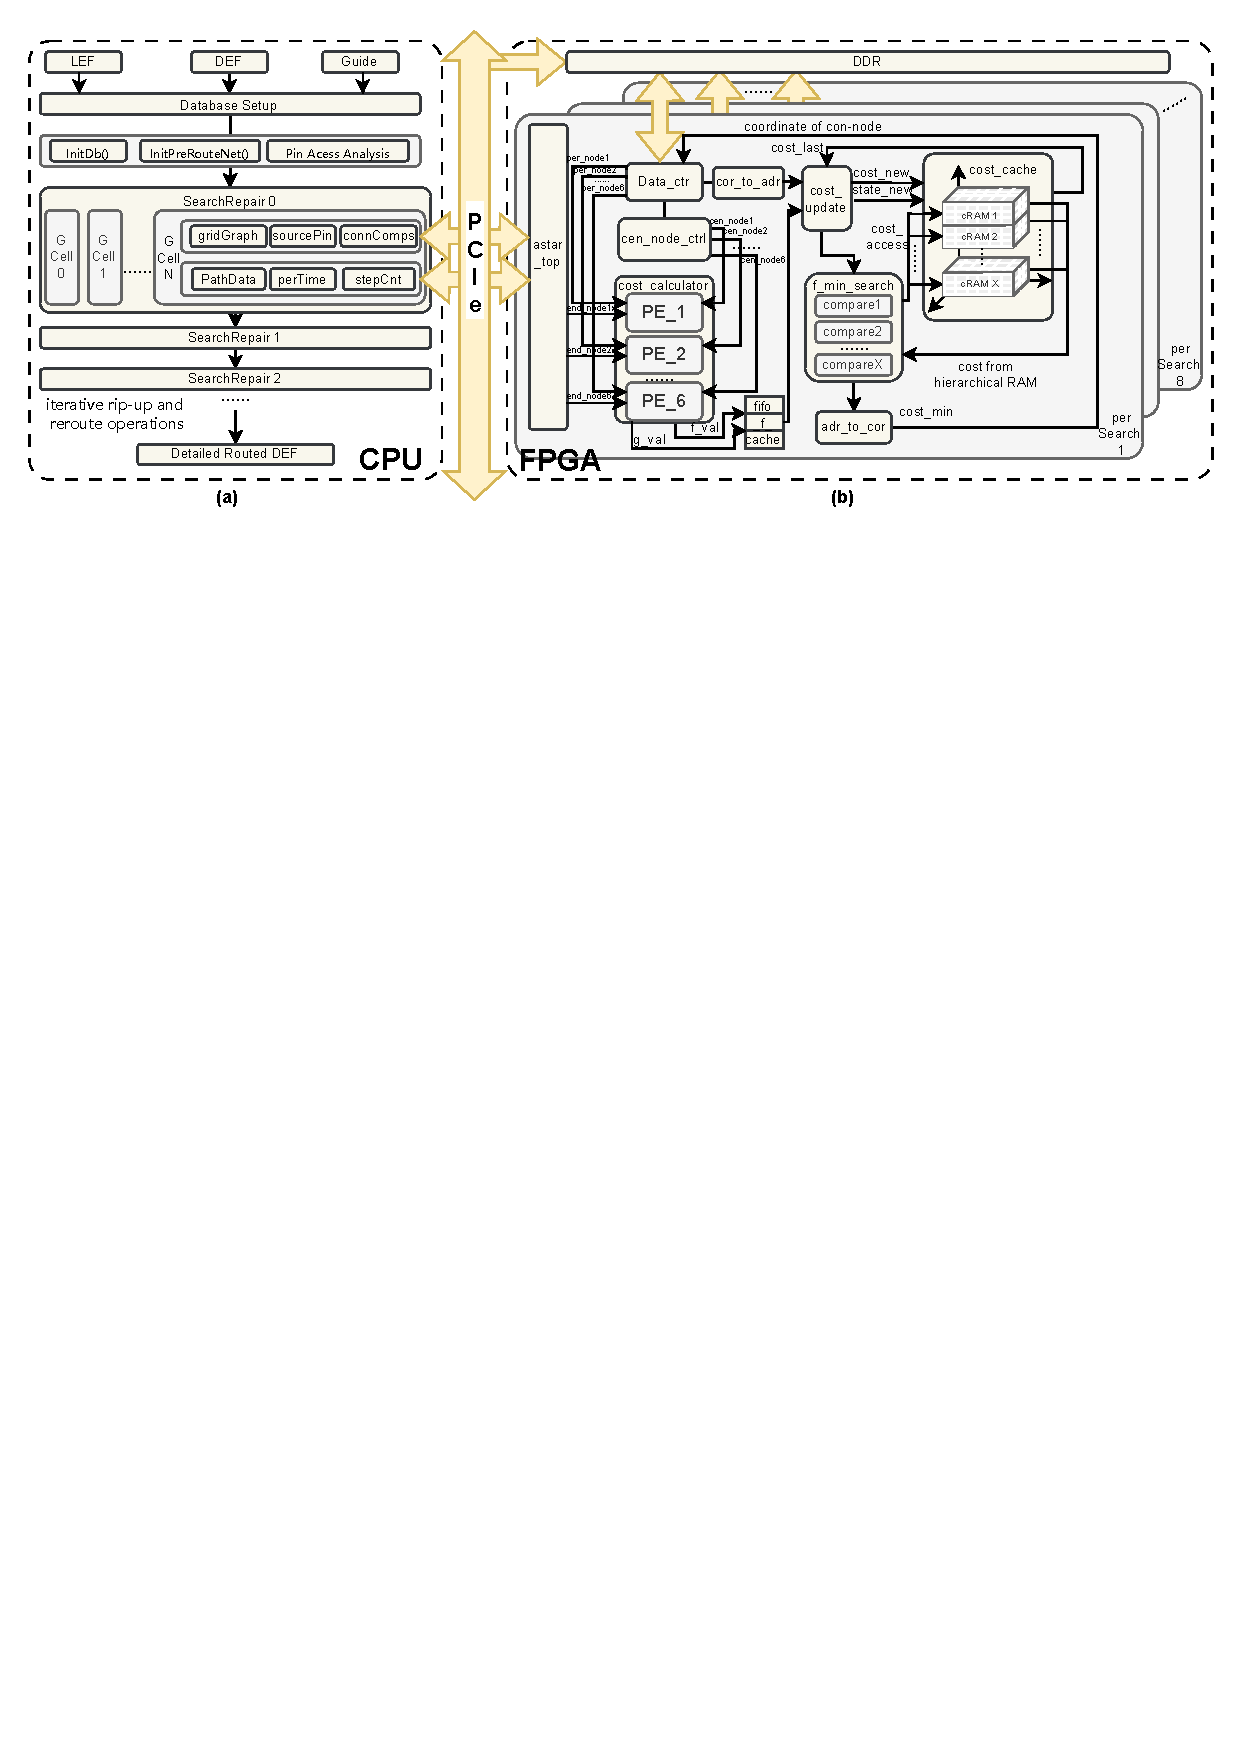
\includegraphics[width=\textwidth]{figures/acceleration/Arch Overview.pdf}
    \caption{The overview structure.(a) The flow of detailed router on GPU.(b) The overview of FPGA acceleration framework.}
    \label{fig:overview} % 标签紧跟标题
\end{figure*}
}

In each round of A* search, we extract the state with the minimum f value from the open list, expand its outer neighbors and check for duplication.
In general, Batched maze routing kernel is executed on a large batch of graphs in the detailed routing stage. There are almost 1,000 ~ 10,000 graphs (nets) in one batch without data dependency between any two graphs, providing a powerful condition for parallelization operation on FPGA to achieve efficient acceleration.

However, the typical maze routing algorithm should be modified to adapt the property of FPGA,as Algorithm 2 shows.
The grid map is initialized in the memory and the start and end nodes are sent to the design so it can start solving the map.
The priority queue Q, the temporary cost set T, and the vertices' state set F used in the hardware-optimized maze routing algorithm are also implemented on hardware.
At the outer level, multiple routing graphs are processed concurrently, exploiting batch-level parallelism with thousands of nets in BRAM.
At the inner level, for each graph, neighbour expansions across multiple directions are executed in parallel to accelerate wavefront propagation.
This fine-grained directional parallelism, combined with hardware-managed cost updates and queue operations, enhances routing throughput on FPGA.

In the process of generating routing diagram, take TritonRoute[?] as an example, through the breadth-first search (BFS) path planning method of extending and updating wavefront, 
the wavefront is dynamically generated and explored in six directions, southeast, northwest and upper, lower, and lower, to gradually update the cost information of each node to realize the path between the target point and the starting point.
It can also be deployed on FPGAs for acceleration through full parallelism and data processing optimization.


%route Split the whole process

%wiring (A* search algorithm is arranged on the FPGA convolution kernel).

%Disassemble and redistribute (compare with the global database, modify the weight), and iterate.

%and the separation of other steps of DRC.

%Processing of database.


% % \subsection{Architecture Design Overview}
% We propose a Mamba accelerator with reconfigurable architecture, \we, with reconfigurable computing units (CUs) and processing elements (PEs).
% \we is a reconfigurable architecture whose instructions are all 64-bit, and contains 16 32-bit general-purpose Registers (Regs) and 16 32-bit Constant Registers (CRegs).
% \we consists of four main parts: instruction processing, normalization unit, on-chip buffer, and computing engine, as depicted in Figure.~\ref{fig:architecture} left.

% \textbf{Instruction Processing.}
% The instruction processing consists of two parts: instruction fetch and instruction decode. 
% The instruction fetch unit fetches instructions from global memory and stores them in the instruction buffer. 
% Then, the instruction decode unit reads instructions sequentially from the buffer and decodes them.
% As shown in Figure~\ref{fig:isa}, the instruction set architecture (ISA) includes linear (\texttt{LIN}), convolution (\texttt{CONV}), normalization (\texttt{NORM}), element-wise multiplication (\texttt{EWM}), element-wise addition (\texttt{EWA}), exponential function (\texttt{EXP}), and SiLU (\texttt{SILU}). 
% And \we also provides \texttt{LOAD} and \texttt{STORE} instructions to support moving data between global memory and on-chip buffer.
% After decoding, the instructions are passed through the configure unit to pass configuration information to the following modules.



% % \textbf{On-chip Buffer.}
% % Buffers are strategically placed throughout the architecture to enhance efficiency. 
% % The buffer pool consists of the input buffer, output buffer, and reconfigurable dual-mode buffer. 
% % The configuration unit determines whether the dual-mode cache serves as an input buffer or an output buffer based on different instructions decoded. 
% % Prior to executing computations, the memory access handler reads data from global memory and writes it into the input buffer for use by computational units. 
% % Intermediate results during computation, as well as the final results, are first written into the output buffer and then transferred to global memory via the memory access handler.


% \textbf{Normalization Unit.}
% The layer normalization is a important component that stabilizes range of intermediate values by normalizing layer activation. 
% The normalization unit is responsible for computing the mean and variance of the data. 
% The data is first summarized and accumulated to get the mean and then the variance is calculated.
% Then, data undergoes a linear unit to obtain the normalized result.

% \textbf{Compute Engine.}
% The compute engine is responsible for linear, convolutional, and element-wise computations. 
% It comprises a control unit and a reconfigurable compute units (RCUs). 
% The control unit receives configuration information from configure unit and fetches data from on-chip buffer to RCU.
% When the computation is completed, it notifies the instruction processing pipeline to continue decoding and executing the next instruction. 


% % \begin{table}[!b]
% % \small
% %   \vspace{-10pt}
% %   \caption{Instruction Set Architecture Definition}
% %   \centering
% %   \vspace{-5pt}
% %   \label{tab:isa}
% %   \begin{tabular}{|l|c|c|c|c|c|}
% %     \hline
% %     \multirow{2}{*}{Operation} & \multirow{2}{*}{Opcode} & Input 0  & Input 1 & Input 1 & Output \\
% %     \multirow{2}{*}{} & \multirow{2}{*}{} & Address & Address & Constant & Address\\
% %     \hline
% %     Linear & 3'b000 & $\checkmark$ & $\checkmark$ & $\checkmark$ & $\checkmark$\\ 
% %     \hline
% %     Conv. & 3'b001 & $\checkmark$ & $\checkmark$ & $\times$ & $\checkmark$ \\ 
% %     \hline
% %     Norm. & 3'b010 & $\checkmark$ & $\times$ & $\times$ & $\checkmark$ \\ 
% %     \hline
% %     Ele. Mul. & 3'b100 & $\checkmark$ & $\checkmark$ & $\checkmark$ & $\checkmark$ \\ 
% %     \hline
% %     Ele. Add. & 3'b101 & $\checkmark$ & $\checkmark$ & $\checkmark$ & $\checkmark$ \\ 
% %     \hline
% %     Ele. Exp. & 3'b110 & $\checkmark$ & $\times$ & $\times$ & $\checkmark$ \\ 
% %     \hline
% %     Ele. SiLU & 3'b111 & $\checkmark$ & $\times$ & $\times$ & $\checkmark$ \\ 
% %   \hline
% % \end{tabular}
% % % \vspace{-10pt}
% % \end{table}

%  \begin{figure*}[!t]
%   \centering
%   \vspace{-5pt}
%   \includegraphics[width=0.98\textwidth]{figures/method1/architecture.pdf}
%   \vspace{-12pt}
%   \caption{Left: Architecture of \we accelerator. \we mainly consists of an instruction processing, a normalization unit, an on-chip buffer,and a compute engine. Middle: Architecture of reconfigurable processing element and reduction tree in RCU. Right: Four reconfigurable modes of RCU, MM-RCU, EW-RCU, EXP-RCU, and SiLU-RCU.}
%   \vspace{-10pt}
%   \label{fig:architecture}
% \end{figure*}

% \begin{figure}[!t]
%   \centering
%   %\vspace{-15pt}
%   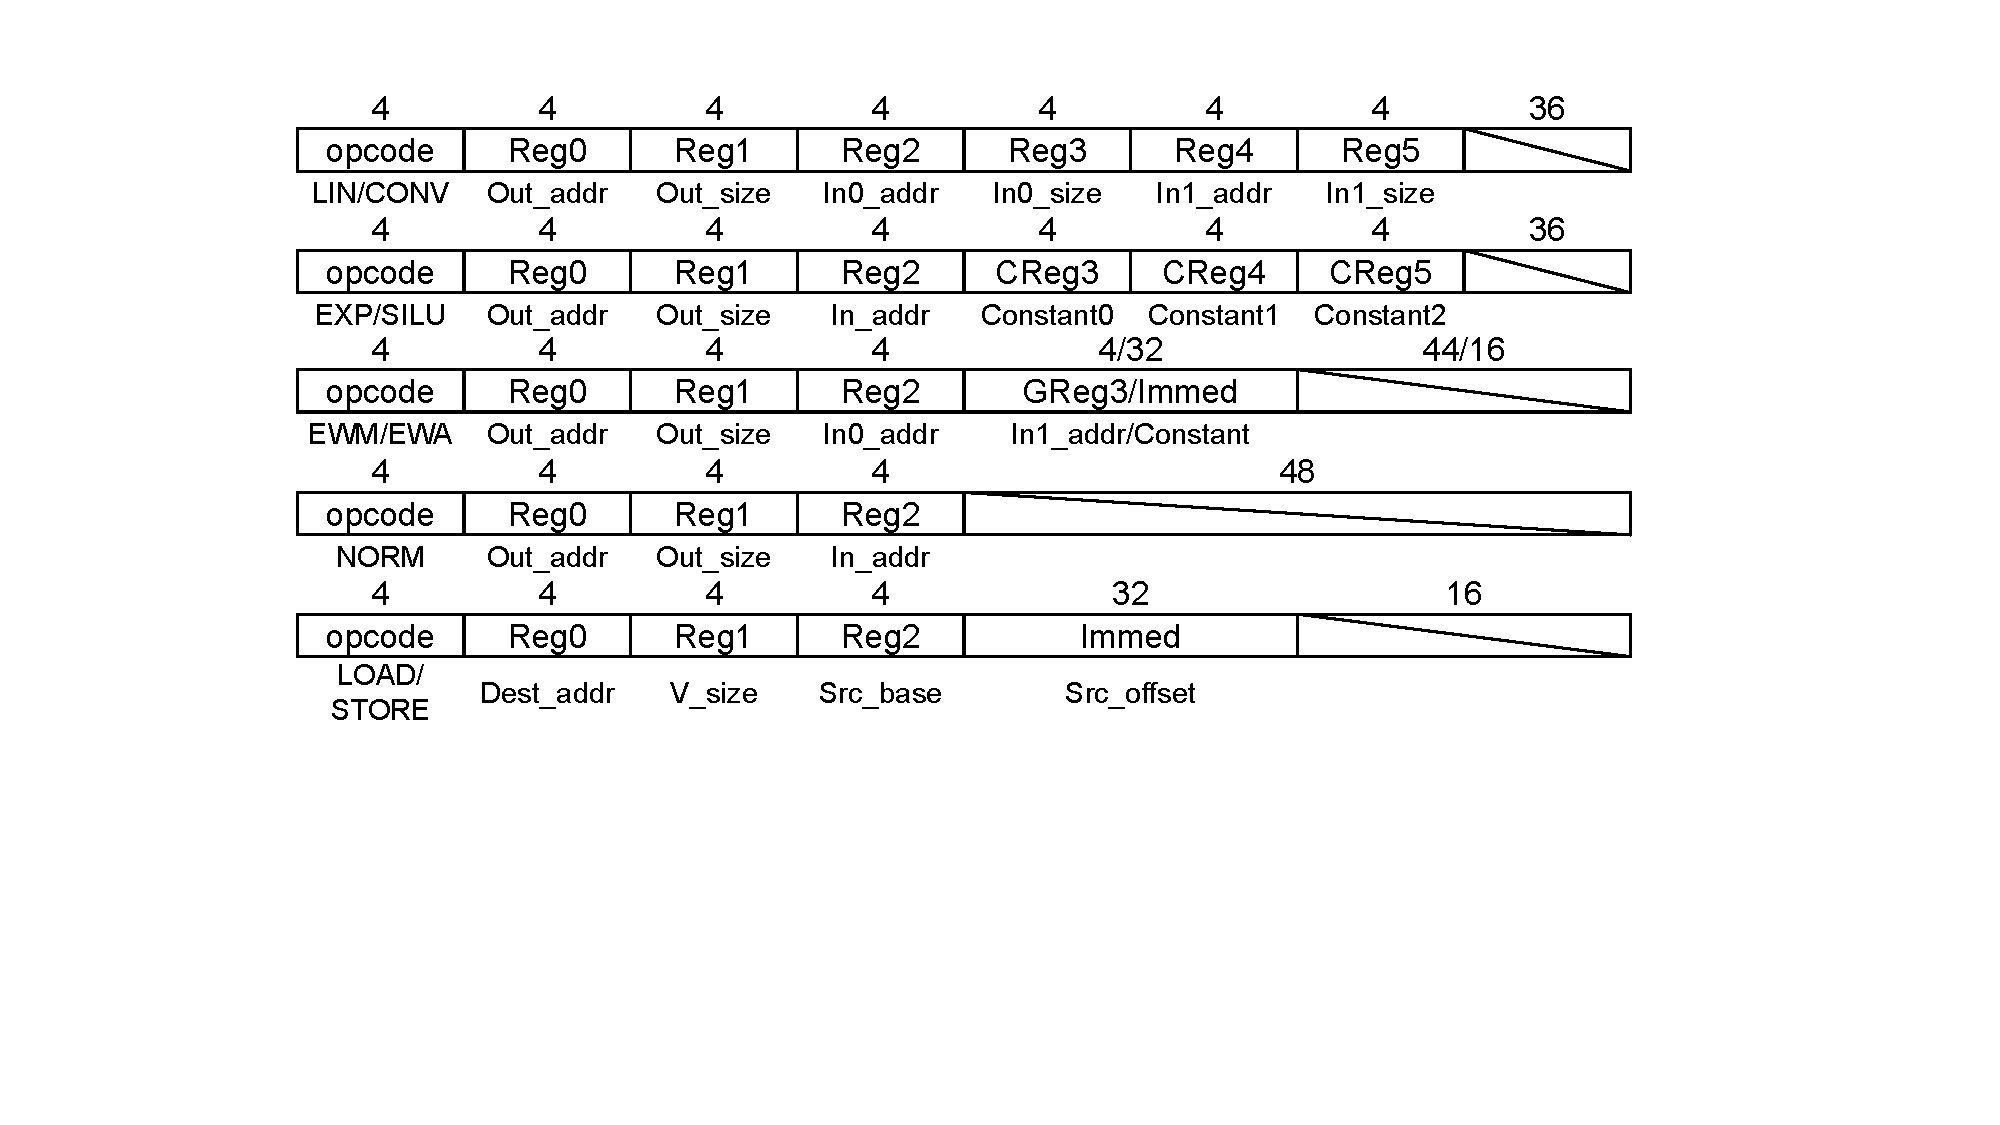
\includegraphics[width=0.48\textwidth]{figures/overview/isa.pdf}
%   \vspace{-18pt}
%   \caption{Instruction set architecture with 16 32-bit general-purpose registers and 16 32-bit constant registers. All instructions are 64-bit.}
%   \vspace{-15pt}
%   \label{fig:isa}
% \end{figure}

% \input{context/arch_overview}

\section{Design of Acceleration Module}
\subsection{The Overview of FPGA Acceleration Framework}
\begin{figure*}[!ht]
    \centering
    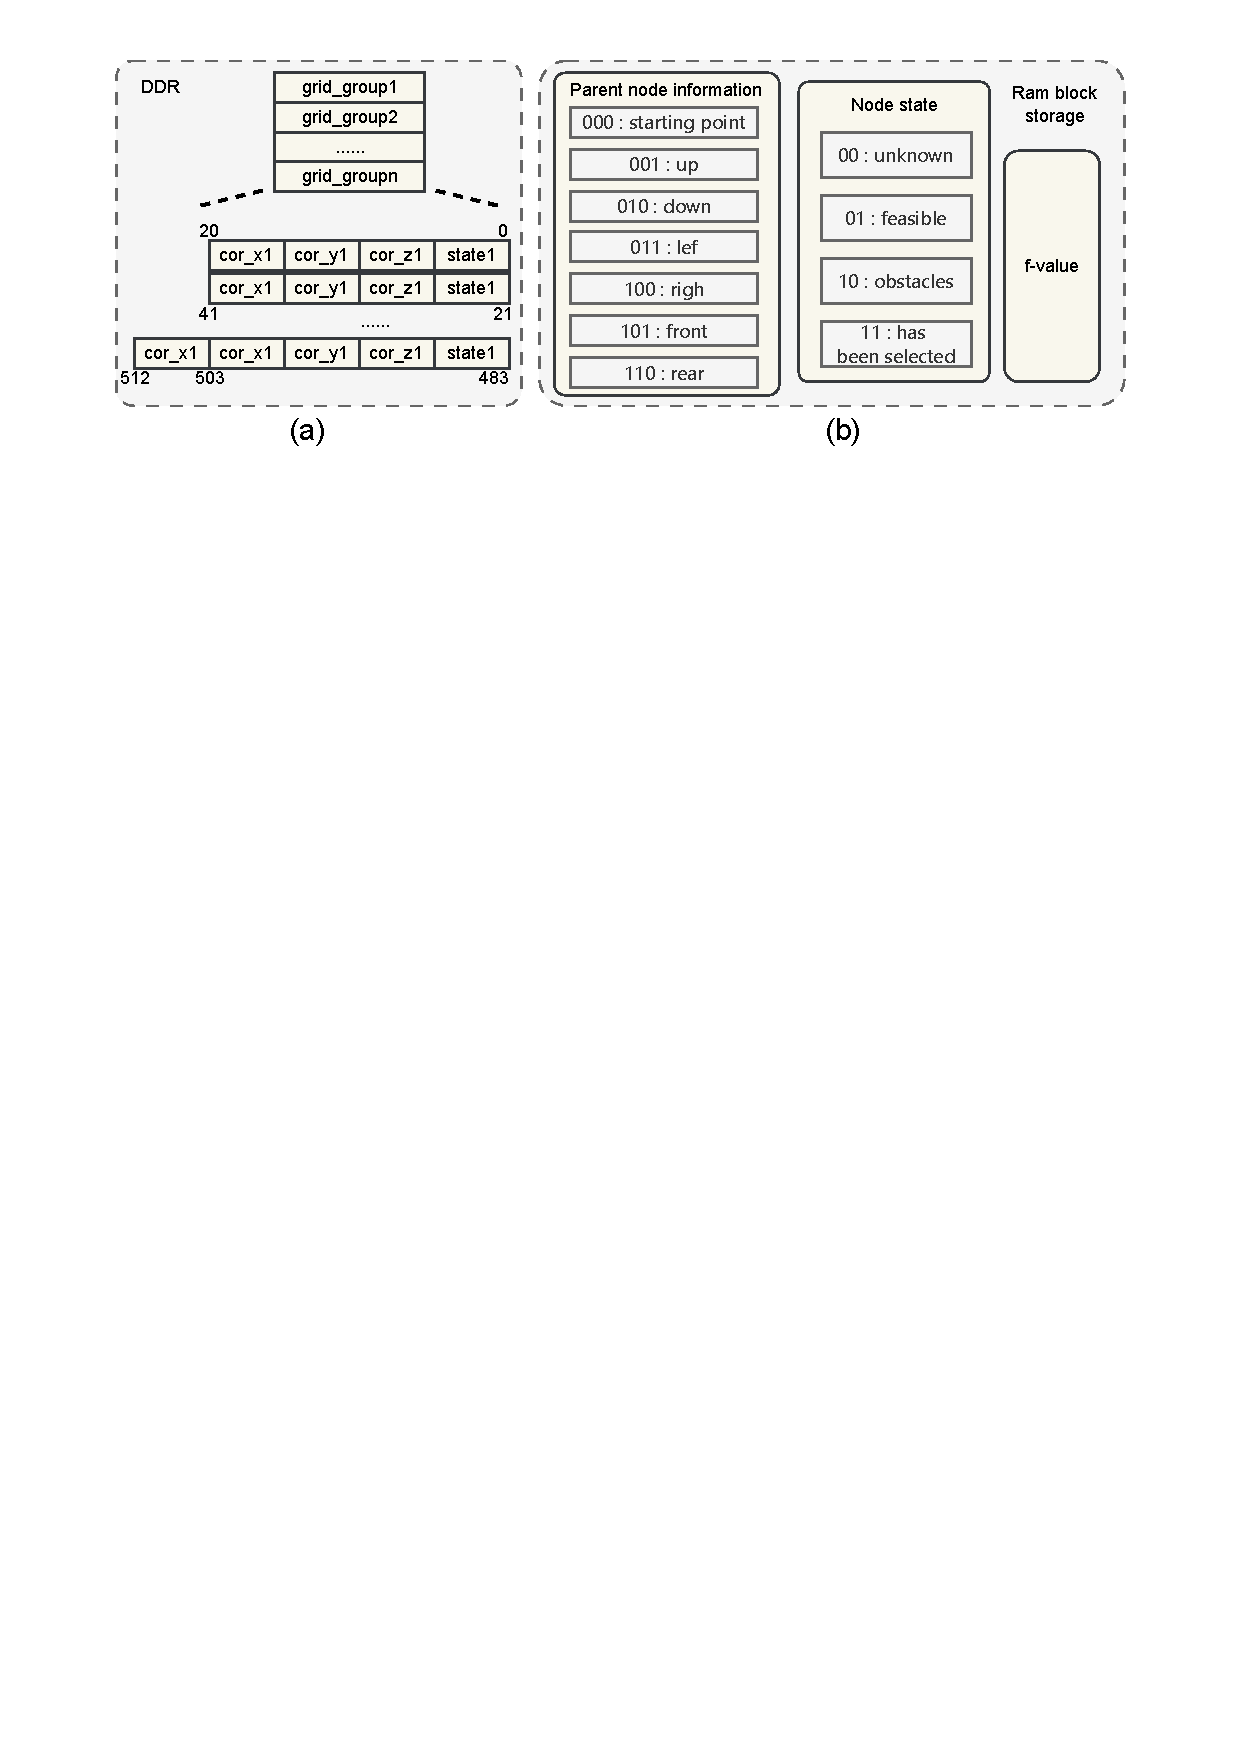
\includegraphics[width=\textwidth]{figures/acceleration/Data Arc.pdf}
    \caption{Data structure ON FPGA.(a)Data Layout in FPGA Memory DDR.(b)Storage format of multi-cRAM.}
\end{figure*}
Conventional implementations of A* search usually use two lists to store the states during its expansion, i.e., the \textbf{open list} and the \textbf{closed list}. 
The closed list stores all the visited states, and is used to prevent unnecessary repeated expansion of the same state. This list is often implemented by a linked hash table to detect the duplicated nodes. 
The open list normally stores the states whose successors have not been fully explored yet. The open list uses a priority queue as its data structure, typically implemented by a binary heap. 
States in the open list are sorted according to the function value of heuristic function f (x).


A lot of work proves that memory access is the time bottleneck of the algorithm compared to the computation time, as Figure~\ref{fig:Execution Time} shows.
So our work is dedicated to propose a FPGA-based implementation to accelerate the detailed routers, uses efficient memory access management and parallelism to achieve better performance.
Figure~\ref{fig:overview} shows the overview of FPGA acceleration framework.





\subsection{Cost\_Calculator Module}
Cost\_calculator module calculates the F-values of 6 peripheral points in parallel according to the input center point and surrounding point information.
The information in 6 directions is calculated in parallel to the Manhattan distance, and the F value of the 6 surrounding points is calculated based on F=G+H.

\begin{figure}[htbp]
    \centering
    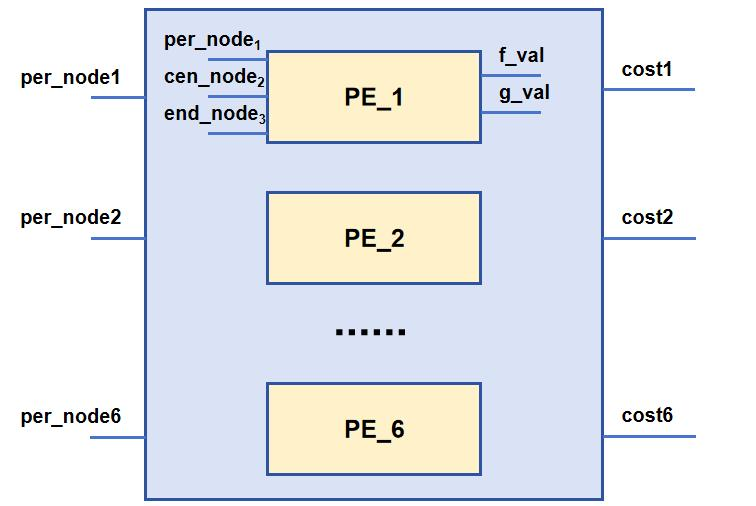
\includegraphics[width=8cm]{figures/acceleration/Cost Calculator Module.jpg}
    \caption{The Cost\_Calculator Module.}
\end{figure}


\subsection{Cost\_Cache Module}
\textbf{Instantiate multiple ram groups to store node information on the corresponding dimension.}Traditional FPGA-based path planning algorithms have significant bottlenecks in maintaining \textbf{open list} and \textbf{closed list}.
The dynamic sorting mechanism requires the storage structure to be reordered after each search iteration. This frequent sorting operation will not only consume a lot of programmable logic resources, but also produce a processing delay that does not match the hardware architecture, which seriously restricts the real-time performance of the system.
In addition, dynamic memory management of variable-length data structures leads to fragmented access to Block RAM, resulting in reduced hardware resource utilization.

To solve this problem we observed, the dimensional organization of RAM can be efficiently managed through hierarchical mapping, in FPGA-based storage architecture design, as fig1 shows.
For 2D data structure, row-priority storage strategy can be adopted, so that each RAM module can store the data node corresponding to the row (first dimension) independently.
When extended to a three-dimensional structure, each RAM module can be responsible for storing node information in a fixed plane, such as the third dimension.
Through the introduction of address mapping module, high-dimensional addresses (such as three-dimensional coordinates (x,y,z)) can be converted into two-dimensional storage addresses inside each RAM module. This hierarchical mapping mechanism significantly improves storage access efficiency and data throughput.





% \begin{table}[]
%     \centering
%     \caption{Ram block storage of node information in the corresponding dimension}
%     \begin{tabular}{|l|l|l|}
%     \hline
%     \multicolumn{1}{|c|}{\textbf{F}} & \multicolumn{1}{c|}{\textbf{Parent node information}} & \multicolumn{1}{c|}{\textbf{Node state}} \\ \hline
%                                       & 000 : starting point                                   & 00 : unknown                               \\ \hline
%                                       & 001 : up                                                & 01 : feasible                              \\ \hline
%                                       & 010 : down                                              & 10 : obstacles                             \\ \hline
%                                       & 011 : left                                              & 11 : has been selected                     \\ \hline
%                                       & 100 : right                                             &                                          \\ \hline
%                                       & 101 : front                                             &                                          \\ \hline
%                                       & 110 : rear                                              &                                          \\ \hline
%     \end{tabular}
%     \end{table}


\begin{figure}[htbp]
    \centering
    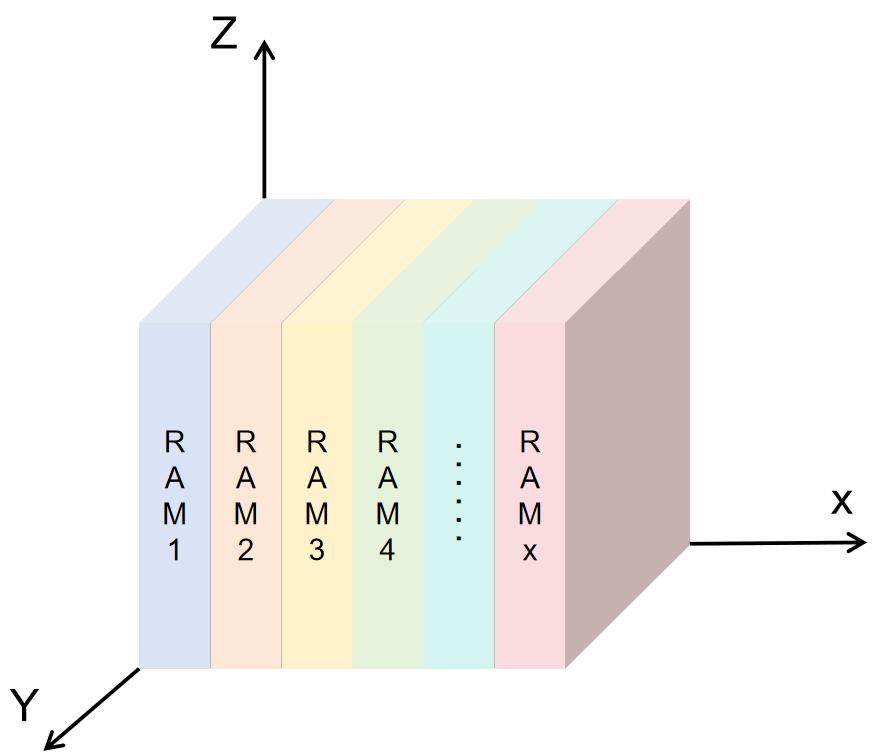
\includegraphics[width=8cm]{figures/acceleration/Cost Cache.jpg}
    \caption{Instantiate multiple ram block storage}
\end{figure}


\subsection{F-value update Module}
After the path cost calculation module completes the F-value generation of the adjacent nodes of the central node, the system executes the storage update process based on logical control.
First, Cost\_cache memory is accessed through the coordinate addressing mechanism to extract the status flag bit and historical F-value of the target node: If the flag bit is detected as the initial state (00), the new F-value and status flag are directly written without constraints;
If the status flag is explored state (01), the hardware comparator is triggered to perform the numerical relationship determination of the new F-value and the stored F-value in parallel, and the path cost validity check is performed at the same time to avoid calculation anomalies.
Finally, the storage unit is selectively updated according to the judgment result: for the initial state node to load new data completely, the explored state node only performs overwrite storage and synchronously updates the state when the new F-value is better.
This mechanism uses the state-driven conditional write strategy to reduce the redundant access to memory and data overwrite operations while maintaining the principle of path planning optimality.

\subsection{Minimum F-Value Sorting Module}
In the process of selecting the least cost node of distributed storage architecture, the system uses the hierarchical comparison mechanism of self-updating to realize the dynamic update of the center point.
The built-in hardware minimum value tracking module of each storage unit immediately triggers the parallel comparison circuit in the unit when a new F-value is detected: real-time comparison of the currently stored minimum F-value and the new written value through the special register group, dynamic update of the minimum cost value and its three-dimensional coordinate information, and generate an effective status flag bit to synchronize to the arbitration controller.
When the valid flag bits of all storage units are ready, the hierarchical comparison architecture starts the global arbitration in stages. First, the local minimum values in each storage row are screened in parallel by row-level comparator array, and then the row-level minimum values are progressively compared by a tree arbiter based on depth-first strategy. Finally, the coordinates and path cost values of the globally optimal nodes are output.

After the selected global minimum is verified, the system loads the new central point information into the path planning logic through the three-dimensional coordinate bus. At the same time, double buffer register group is used to realize the decoupling of the computing unit and the storage unit to ensure the continuous operation of the comparison pipeline during the data update cycle.
By means of distributed priority arbitration mechanism implemented by hardware, the architecture transforms the ergodic search in traditional algorithms into multilevel pipeline operation, which avoids the resource competition problem of centralized comparison architecture while maintaining real-time path planning.
% \section{Reduction Alternative PE Array Architecture}\label{sec:method1}

% \subsection{Challenge}

% Linear operation and element-wise operation are two dominating operations in Mamba.
% Linear operations like matrix multiplications are usually accelerated by Tensor Core, which is a domain specific architecture with the reduction tree.
% Due to the reduction of partial inner product, the linear operations exhibit extremely high compute intensity (\textit{e.g.}, $>$1000 FLOPs/Byte).
% However, as shown in Figure~\ref{fig:time_proportion}, the time proportion of element-wise operations escalates significantly as sequence length increases (\textit{e.g.}, $>$60\% with 2048 input length).
% Because the element-wise operations do not need reduction, applying them on Tensor Core-based architecture should introduce large amount of invalid computations, leading to an extreme inefficiency (\textit{e.g.}, 1/16 normalized speed). 
% We call it the incompatibility between element-wise operations and Tensor Core.

% \subsection{Motivation and Insights}

% Our motivation stems from the inefficiencies observed in element-wise computations on tensor cores. 
% Because the attention operations contain non-linear softmax, previous Transformer accelerators~\cite{wang2022via,lu2020hardware} employed independent hardware units to support both attention and linear operations. 
% In contrast, Mamba architecture only consists of linear operations, element-wise operations, and a few activation functions. 
% The only difference of linear of element-wise operations is whether execute reduction or not. 
% Recognizing this simplicity, \textbf{our key insight is that by disabling the reduction tree, the Tensor Core-based PE arrays can execute element-wise operations.}
% % Recognizing this simplicity, our key insight lies in the integration of hardware units capable of handling these dominant linear and element-wise operations, thereby maximizing hardware reuse.

% \subsection{Approach}
% \textbf{Reduction Alternative PE Arrays.}
% The reduction alternative processing element (PE) arrays support configurablility. 
% The reduction tree consists of 16 slices (taking 16 for instance) and operates in two modes: reduction mode for linear operations and non-reduction mode for element-wise operations. 
% In reduction mode, the reduction tree is enabled.
% For a 16-to-1 reduction tree slice, the outputs from 16$\times$1 PE arrays are fed into one reduction tree slice, which employs multi-level additions to compute the sum.
% In non-reduction mode, the reduction tree is enabled and the outputs from 16$\times$16 PE arrays skip the reduction directly. 
% In addition, the last-level addition in each slice supports three input to accumulate the partial results for linear operations.

% We define that a reconfigurable computing unit (RCU) consists of  16$\times$16 PE arrays and a reduction tree, as shown in Figure~\ref{fig:architecture} left. 
% Each reconfigurable PE (RPE) is configured to support three main computations with three data paths: a shift path for exponential function, a piecewise path for SiLU function, and a normal path for addition or multiplication. 
% The normal path contains a floating-point multiplier, a floating-point adder, and a multiplexer unit to handle element-wise multiplication and addition computations. 
 

% \textbf{Reconfigurable Computing Unit.}
% We provide a detailed explanation of how the RCU operates for the four specific computations in Mamba, as shown in Figure~\ref{fig:architecture} right.

% \textit{\underline{MM-RCU.}}
% The RCU is configured as a matrix multiplication mode (MM-RCU) to support linear operations. 
% The reduction tree in RCU and the floating-point multiplier units in RPE are enabled. 
% Therefore, for a matrix multiplication operation of two matrices of size 16$\times$16, the results calculated by the 16$\times$16 array of multipliers are then passed through the reduction tree to produce 16 final results. 
% Then, this process is repeated totally 16 times to obtain the complete result of the 16$\times$16 matrix multiplication. 
% To support the accumulation of partial sums, an additional adder is added at the final level of the reduction tree.

% \textit{\underline{EW-RCU.}}
% When RCU is configured as element-wise mode (EW-RCU), the reduction tree is disabled, while the P2D buffer is enabled, and the floating-point multiplier or adder units in RPE are activated. 
% For an element-wise multiplication operation of two 16x16 matrices, the results calculated by the 16$\times$16 array of RPEs maintains the same dimensions of 16$\times$16 and are output to the buffer in parallel.
% % After 16 clock cycles, the results are sequentially written out.

% \textit{\underline{EXP-RCU.}}
% When RCU is configured as exponential mode (EXP-RCU), the reduction tree is disabled. 
% The floating-point multiplier, adder units, and exponential shift unit in RPE are enabled. 
% Therefore, for a 16$\times$16 matrix performing exponential function operation, the RCU first executes element-wise multiplication by using the multipliers, then executes element-wise addition by using the adders. 
% Afterward, the exponential shift unit performs a logic operation, a shift operation and a biased operation to obtain the final output, as shown in Figure~\ref{fig:overview} right bottom.

% \textit{\underline{SiLU-RCU.}}
% When RCU is configured as SiLU mode (SiLU-RCU), the floating-point multiplier or adder, the range detector, and the constant output unit in RPE are enabled while the reduction tree is disabled.
% For a 16$\times$16 input matrix, each input is first distinguished by range, and then depending on the difference of range, each input is processed by employing either the constant output or normal element-wise computations.
% The SiLU-RCU decomposes the SiLU operation into 0, 2, or 4 instances of element-wise operations according to equation~\ref{eq:silu_approx}.


% \section{Reusable Nonlinear Function Unit}\label{sec:method3}


% \subsection{Challenge}
% Exponential function and Sigmoid Linear Unit (SiLU) function are two nonlinear functions in Mamba. 
% Previous methods~\cite{exp_unit,nilsson2014hardware,reggiani2023flex} often design specific unit based on lookup-table or Taylor series approximation to optimize these nonlinear computations.
% However, the optimized nonlinear function unit such exponential function still occupy 30\% of the PE area~\cite{exp_unit,tstc}, leading to much more area overheads.


% \subsection{Motivation and Insights}
% A common approach is to utilize approximation functions to approximate exponential operations, thereby degrading exponential computations to quadratic or even linear operations.
% Using linear approximation methods results in large precision loss ($>$4\% for Mamba-2.8b) while employing higher-order polynomial approximation leads to increased computational overhead.
% We profile the range of these nonlinear functions.
% The input for an exponential function is mostly between -7 and 0, especially for values slightly less than 0,
% while the input range of the SiLU function is from -5 to 4.
% On one hand, we can only approximate nonlinear functions only in these range to concentrate on preventing accuracy loss.
% On the other hand, exponential function and SiLU are similar with element-wise operations except for scaling for each value. 
% Therefore, to avoid increasing area overhead and prevent accuracy loss, our key insight is that \textbf{only by approximating these nonlinear functions in a small range, we can decompose them into several element-wise operations to reuse the reduction alternative PE array architecture in Section~\ref{sec:method1}.}


% \subsection{Approach}

% \textbf{Fast Biased Exponential Algorithm.}
% Given the peculiar distribution observed in the inputs of the exponential function, namely the outer product of $\Delta$ and A, we leverage a set of data points $x=\frac{-7}{n}, n=1,2,...,200$ where the density increases as they approach zero to evaluate the deviation of the approximate calculation from the origin exponential value. Consequently, we modified the fast exp algorithm~\cite{fast_exp} to accommodate specific data ranges and appended a bias at the end to enhance precision and consists of three main steps:

% \begin{enumerate}
%     \item The input \( x \) is linearly transformed into \( x' \).
%     \item \( x' \) is multiplied by $2^{23}$ then cast to an unsigned integer.
%     \item View the x as float-point number and add the bias \( c \).
% \end{enumerate}
%  The fast exp algorithm aims to put $\frac{x}{ln2}$ into exponential bit of $e^{x}$ so that $e^{x} = 2^{\left(\frac{x}{ln2}\right)}$. Float data does not have a direct intuitive representation like unsigned integers, hence cannot be directly used as the exponent bits for $e^{x}$; therefore, conversion to uint is necessary. Additionally, a bias is required to compensate for conversion loss. The exponent of a float is typically subtracted by 127 during actual computations so we also need consider that. Now we can determine the coefficient \(a = \frac{1}{\ln(2)}\) and the term \(b = 127 + bias\), while \(c\) serves as the final bias, effectively reducing the average loss caused by specific data distributions.

% \begin{figure}[!t]
%     \centering
%     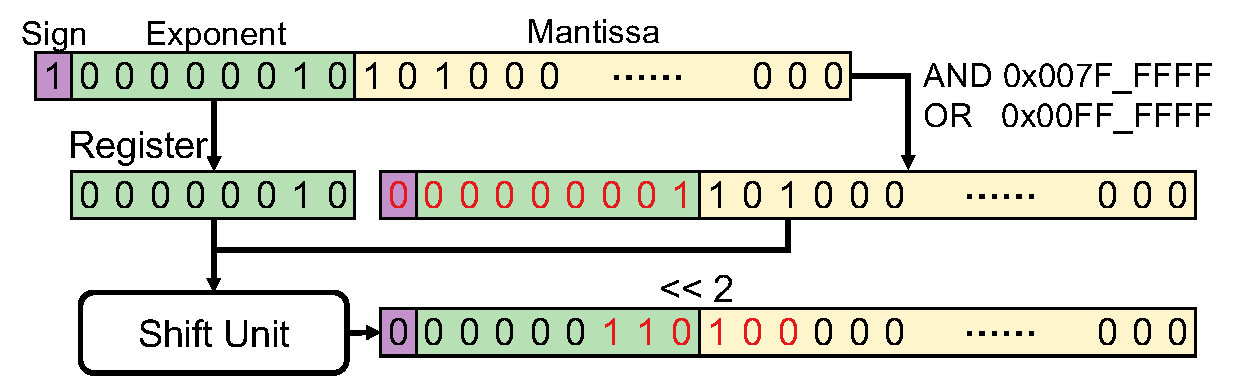
\includegraphics[width=0.48\textwidth]{figures/method3/exp_cast_unit.pdf}
%     \vspace{-20pt}
%     \caption{Hardware implementation of exponential shift unit for our fast exponential approximation.}
%     \vspace{-18pt}
%     \label{fig:approximation}
% \end{figure}

% % \subsection{Approach: SiLU Approximation}
% \textbf{Piecewise SiLU Algorithm.}
% The computational formula for the SiLU function is $SiLU(x) = x\cdot \sigma(x) = \frac{x}{1 + e^{-x}}$
% which involves not only exponentiation but also division operations. Though employing the fast exp algorithm for approximation yields excellent precision, it introduces overhead due to the need for dividers, consequently impacting performance. Our preliminary profiling results indicate that the inputs to the SiLU function are mostly concentrated in the range [-5, 4]. Therefore, we propose segmenting the SiLU function within this interval for approximation. Increasing the number of segments enhances precision but also introduces more conditional branches, thus impacting performance. Consequently, we strike a balance between precision and performance and utilize a 4-segment piecewise function to approximate the SiLU function which is expressed by equation \ref{eq:silu_approx}: Within each interval, further piece-wise approximation is performed based on the distribution of the data.

% \begin{equation}\label{eq:silu_approx}
% f(x) = \left\{
% \begin{aligned}
%     &-0.0135, && \text{if } x < -5 \\
%     &-0.06244x - 0.3457, && \text{if } -5 \leq x < -1.5 \\
%     &0.232(x + 1.181)^{2} - 0.275, && \text{if } -1.5 \leq x \leq 0.75 \\
%     &1.05x - 0.2781, && \text{if } x > 0.75
% \end{aligned}
% \right.
% \end{equation}

% % \subsection{Approach: Hardware Implementation}
% \textbf{Reusable Nonlinear Function Unit.}
% Based on two algorithms for nonlinear functions, we decompose the exponential function into element-wise operations and an shift operation, and SiLU into a range detection and element-wise operations.
% Therefore, we only add a few logics and resue PE arrays to support nonlinear  functions.

% \textit{\underline{As Exponential Function Unit.}} The original computation process of fast exp is overly complex, particularly the float-to-uint conversion unit incurring significant overhead, we have devised a dedicated conversion unit shown in Figure \ref{fig:approximation} for fast exp. Within this unit, the input \( x \) undergoes floating-point linear computation, resulting in \( x' \). Subsequently, we extract the 8 exponent bits of \( x' \), directly representing the required shift length—positive for left shifts and negative for right shifts. Next, employing logical operations, we convert the original floating-point number into the actual representation of the mantissa. Finally, the result is fed into a shift unit and adjusted through a bias unit to yield the output. Due to the ability to simplify the series of linear transformations applied to the input into a single linear transformation, the actual computation only requires 4 cycles.
% % \item 

% \textit{\underline{As SiLU Unit.}} The SiLU unit introduces a range detector in the PE unit, responsible for determining the input's interval and executing the corresponding computation. Due to the most complex operation being quadratic, the actual computational overhead is minimal.
% % \end{itemize}

% % By employing the approximation algorithm, We can eliminate the exponential units and divider within the PE, replacing them with an efficient linear computation flow.


\section{Experimental Results}\label{sec:experiment}
\subsection{Experimental Setup}

CPU:Intel(R) Xeon(R) Gold 5218R CPU @ 2.10GHz,Memory:64G,8Thread;FPGA, xcvu9p,8 computing cores in parallel


\subsection{Maze Routing Acceleration}

% Please add the following required packages to your document preamble:
% \usepackage{multirow}
% \begin{table*}[!htbp]
%     \caption{Comparison of performance between TritonRoute [?] Dr.CU and our FPGA acceleration to complete batched maze routing kernel with ISPD 2018 [?] contest benchmarks.}
%     \begin{tabular}{|c|ccll|clll|llll|lllc|cccl|cl|}
%     \hline
%     \multirow{2}{*}{Benchmark} & \multicolumn{4}{c|}{Wirelength(um)}                                                                             & \multicolumn{4}{c|}{Via count}                                                                                  & \multicolumn{4}{c|}{Memory(GB)}                                                                                 & \multicolumn{4}{c|}{\begin{tabular}[c]{@{}c@{}}ISPD' 18 \\ quality score\end{tabular}}     & \multicolumn{4}{c|}{\begin{tabular}[c]{@{}c@{}}Routing Kernel\\ Runtime(s)\end{tabular}}                            & \multicolumn{2}{c|}{\begin{tabular}[c]{@{}c@{}}Routing Kernel\\ Speed-up\end{tabular}} \\ \cline{2-23} 
%                                & \multicolumn{1}{c|}{TR} & \multicolumn{1}{c|}{CU} & \multicolumn{1}{c|}{MAcc-TR} & \multicolumn{1}{c|}{MAcc-CU} & \multicolumn{1}{c|}{TR} & \multicolumn{1}{c|}{CU} & \multicolumn{1}{c|}{MAcc-TR} & \multicolumn{1}{c|}{MAcc-CU} & \multicolumn{1}{c|}{TR} & \multicolumn{1}{c|}{CU} & \multicolumn{1}{c|}{MAcc-TR} & \multicolumn{1}{c|}{MAcc-CU} & \multicolumn{1}{c|}{TR} & \multicolumn{1}{c|}{CU} & \multicolumn{1}{c|}{MAcc-TR} & MAcc-CU & \multicolumn{1}{c|}{TR}     & \multicolumn{1}{c|}{CU} & \multicolumn{1}{c|}{MAcc-TR} & \multicolumn{1}{c|}{MAcc-CU} & \multicolumn{1}{c|}{MAcc-TR}               & \multicolumn{1}{c|}{MAcc-CU}              \\ \hline
%     ispd18\_testl              & \multicolumn{1}{c|}{}   & \multicolumn{1}{c|}{}   & \multicolumn{1}{l|}{}        &                              & \multicolumn{1}{c|}{}   & \multicolumn{1}{l|}{}   & \multicolumn{1}{l|}{}        &                              & \multicolumn{1}{l|}{}   & \multicolumn{1}{l|}{}   & \multicolumn{1}{l|}{}        &                              & \multicolumn{1}{l|}{}   & \multicolumn{1}{l|}{}   & \multicolumn{1}{l|}{}        &         & \multicolumn{1}{c|}{4.41}   & \multicolumn{1}{c|}{}   & \multicolumn{1}{c|}{2.03}    &                              & \multicolumn{1}{c|}{2.2x}                  &                                           \\ \hline
%     ispd18\_test2              & \multicolumn{1}{c|}{}   & \multicolumn{1}{c|}{}   & \multicolumn{1}{l|}{}        &                              & \multicolumn{1}{c|}{}   & \multicolumn{1}{l|}{}   & \multicolumn{1}{l|}{}        &                              & \multicolumn{1}{l|}{}   & \multicolumn{1}{l|}{}   & \multicolumn{1}{l|}{}        &                              & \multicolumn{1}{l|}{}   & \multicolumn{1}{l|}{}   & \multicolumn{1}{l|}{}        &         & \multicolumn{1}{c|}{58.86}  & \multicolumn{1}{c|}{}   & \multicolumn{1}{c|}{25.93}   &                              & \multicolumn{1}{c|}{2.3x}                  &                                           \\ \hline
%     ispd18\_test3              & \multicolumn{1}{c|}{}   & \multicolumn{1}{c|}{}   & \multicolumn{1}{l|}{}        &                              & \multicolumn{1}{c|}{}   & \multicolumn{1}{l|}{}   & \multicolumn{1}{l|}{}        &                              & \multicolumn{1}{l|}{}   & \multicolumn{1}{l|}{}   & \multicolumn{1}{l|}{}        &                              & \multicolumn{1}{l|}{}   & \multicolumn{1}{l|}{}   & \multicolumn{1}{l|}{}        &         & \multicolumn{1}{c|}{110.07} & \multicolumn{1}{c|}{}   & \multicolumn{1}{c|}{52.4}    &                              & \multicolumn{1}{c|}{2.1x}                  &                                           \\ \hline
%     ispd18\_test4              & \multicolumn{1}{c|}{}   & \multicolumn{1}{c|}{}   & \multicolumn{1}{l|}{}        &                              & \multicolumn{1}{c|}{}   & \multicolumn{1}{l|}{}   & \multicolumn{1}{l|}{}        &                              & \multicolumn{1}{l|}{}   & \multicolumn{1}{l|}{}   & \multicolumn{1}{l|}{}        &                              & \multicolumn{1}{l|}{}   & \multicolumn{1}{l|}{}   & \multicolumn{1}{l|}{}        &         & \multicolumn{1}{c|}{244.48} & \multicolumn{1}{c|}{}   & \multicolumn{1}{c|}{211.68}  &                              & \multicolumn{1}{c|}{2.3x}                  &                                           \\ \hline
%     ispd18\_test5              & \multicolumn{1}{c|}{}   & \multicolumn{1}{c|}{}   & \multicolumn{1}{l|}{}        &                              & \multicolumn{1}{c|}{}   & \multicolumn{1}{l|}{}   & \multicolumn{1}{l|}{}        &                              & \multicolumn{1}{l|}{}   & \multicolumn{1}{l|}{}   & \multicolumn{1}{l|}{}        &                              & \multicolumn{1}{l|}{}   & \multicolumn{1}{l|}{}   & \multicolumn{1}{l|}{}        &         & \multicolumn{1}{c|}{109.42} & \multicolumn{1}{c|}{}   & \multicolumn{1}{c|}{40.39}   &                              & \multicolumn{1}{c|}{2.3x}                  &                                           \\ \hline
%     ispd18\_test6              & \multicolumn{1}{c|}{}   & \multicolumn{1}{c|}{}   & \multicolumn{1}{l|}{}        &                              & \multicolumn{1}{c|}{}   & \multicolumn{1}{l|}{}   & \multicolumn{1}{l|}{}        &                              & \multicolumn{1}{l|}{}   & \multicolumn{1}{l|}{}   & \multicolumn{1}{l|}{}        &                              & \multicolumn{1}{l|}{}   & \multicolumn{1}{l|}{}   & \multicolumn{1}{l|}{}        &         & \multicolumn{1}{c|}{165.39} & \multicolumn{1}{c|}{}   & \multicolumn{1}{c|}{77.33}   &                              & \multicolumn{1}{c|}{2.1x}                  &                                           \\ \hline
%     ispd18\_test7              & \multicolumn{1}{c|}{}   & \multicolumn{1}{c|}{}   & \multicolumn{1}{l|}{}        &                              & \multicolumn{1}{c|}{}   & \multicolumn{1}{l|}{}   & \multicolumn{1}{l|}{}        &                              & \multicolumn{1}{l|}{}   & \multicolumn{1}{l|}{}   & \multicolumn{1}{l|}{}        &                              & \multicolumn{1}{l|}{}   & \multicolumn{1}{l|}{}   & \multicolumn{1}{l|}{}        &         & \multicolumn{1}{c|}{246.12} & \multicolumn{1}{c|}{}   & \multicolumn{1}{c|}{111.98}  &                              & \multicolumn{1}{c|}{2.2x}                  &                                           \\ \hline
%     ispd18\_test8              & \multicolumn{1}{c|}{}   & \multicolumn{1}{c|}{}   & \multicolumn{1}{l|}{}        &                              & \multicolumn{1}{c|}{}   & \multicolumn{1}{l|}{}   & \multicolumn{1}{l|}{}        &                              & \multicolumn{1}{l|}{}   & \multicolumn{1}{l|}{}   & \multicolumn{1}{l|}{}        &                              & \multicolumn{1}{l|}{}   & \multicolumn{1}{l|}{}   & \multicolumn{1}{l|}{}        &         & \multicolumn{1}{c|}{256.73} & \multicolumn{1}{c|}{}   & \multicolumn{1}{c|}{125.29}  &                              & \multicolumn{1}{c|}{2.1x}                  &                                           \\ \hline
%     ispd18\_test9              & \multicolumn{1}{c|}{}   & \multicolumn{1}{c|}{}   & \multicolumn{1}{l|}{}        &                              & \multicolumn{1}{c|}{}   & \multicolumn{1}{l|}{}   & \multicolumn{1}{l|}{}        &                              & \multicolumn{1}{l|}{}   & \multicolumn{1}{l|}{}   & \multicolumn{1}{l|}{}        &                              & \multicolumn{1}{l|}{}   & \multicolumn{1}{l|}{}   & \multicolumn{1}{l|}{}        &         & \multicolumn{1}{c|}{264.21} & \multicolumn{1}{c|}{}   & \multicolumn{1}{c|}{128.19}  &                              & \multicolumn{1}{c|}{2.1x}                  &                                           \\ \hline
%     ispd18\_test10             & \multicolumn{1}{c|}{}   & \multicolumn{1}{c|}{}   & \multicolumn{1}{l|}{}        &                              & \multicolumn{1}{c|}{}   & \multicolumn{1}{l|}{}   & \multicolumn{1}{l|}{}        &                              & \multicolumn{1}{l|}{}   & \multicolumn{1}{l|}{}   & \multicolumn{1}{l|}{}        &                              & \multicolumn{1}{l|}{}   & \multicolumn{1}{l|}{}   & \multicolumn{1}{l|}{}        &         & \multicolumn{1}{c|}{380.69} & \multicolumn{1}{c|}{}   & \multicolumn{1}{c|}{180.455} &                              & \multicolumn{1}{c|}{2.1x}                  &                                           \\ \hline
%     \end{tabular}
%     \label{tab:wide_table}
%     \end{table*}
% Please add the following required packages to your document preamble:
% \usepackage{multirow}
% Please add the following required packages to your document preamble:
% \usepackage{multirow}
% \begin{table*}[!htbp]
%     \centering
%     \caption{Comparison of performance between TritonRoute [?] Dr.CU and our FPGA acceleration to complete batched maze routing kernel with ISPD 2018 [?] contest benchmarks.}
%     \begin{tabularx}{\textwidth}{|c|ccll|clll|lllc|cccl|cl|}
%     \hline
%     \multirow{2}{*}{ispd18} & \multicolumn{4}{c|}{Wirelength(um)}                                                                                                                                                                   & \multicolumn{4}{c|}{Via count}                                                                                                                                                                        & \multicolumn{4}{c|}{\begin{tabular}[c]{@{}c@{}}ISPD' 18 \\ quality score\end{tabular}}                                                                                           & \multicolumn{4}{c|}{\begin{tabular}[c]{@{}c@{}}Routing Kernel\\ Runtime(s)\end{tabular}}                                                                                                                  & \multicolumn{2}{c|}{\begin{tabular}[c]{@{}c@{}}Routing Kernel\\ Speed-up\end{tabular}}                                                            \\ \cline{2-19} 
%                             & \multicolumn{1}{c|}{TR} & \multicolumn{1}{c|}{CU} & \multicolumn{1}{c|}{\begin{tabular}[c]{@{}c@{}}MAcc\\ -TR\end{tabular}} & \multicolumn{1}{c|}{\begin{tabular}[c]{@{}c@{}}MAcc\\ -CU\end{tabular}} & \multicolumn{1}{c|}{TR} & \multicolumn{1}{c|}{CU} & \multicolumn{1}{c|}{\begin{tabular}[c]{@{}c@{}}MAcc\\ -TR\end{tabular}} & \multicolumn{1}{c|}{\begin{tabular}[c]{@{}c@{}}MAcc\\ -CU\end{tabular}} & \multicolumn{1}{c|}{TR} & \multicolumn{1}{c|}{CU} & \multicolumn{1}{c|}{\begin{tabular}[c]{@{}c@{}}MAcc\\ -TR\end{tabular}} & \begin{tabular}[c]{@{}c@{}}MAcc\\ -CU\end{tabular} & \multicolumn{1}{c|}{TR}     & \multicolumn{1}{c|}{CU} & \multicolumn{1}{c|}{\begin{tabular}[c]{@{}c@{}}MAcc\\ -TR\end{tabular}} & \multicolumn{1}{c|}{\begin{tabular}[c]{@{}c@{}}MAcc\\ -CU\end{tabular}} & \multicolumn{1}{c|}{\begin{tabular}[c]{@{}c@{}}MAcc\\ -TR\end{tabular}} & \multicolumn{1}{c|}{\begin{tabular}[c]{@{}c@{}}MAcc\\ -CU\end{tabular}} \\ \hline
%     testl                   & \multicolumn{1}{c|}{}   & \multicolumn{1}{c|}{}   & \multicolumn{1}{l|}{}                                                   &                                                                         & \multicolumn{1}{c|}{}   & \multicolumn{1}{l|}{}   & \multicolumn{1}{l|}{}                                                   &                                                                         & \multicolumn{1}{l|}{}   & \multicolumn{1}{l|}{}   & \multicolumn{1}{l|}{}                                                   &                                                    & \multicolumn{1}{c|}{4.41}   & \multicolumn{1}{c|}{}   & \multicolumn{1}{c|}{2.03}                                               &                                                                         & \multicolumn{1}{c|}{2.2x}                                               &                                                                         \\ \hline
%     test2                   & \multicolumn{1}{c|}{}   & \multicolumn{1}{c|}{}   & \multicolumn{1}{l|}{}                                                   &                                                                         & \multicolumn{1}{c|}{}   & \multicolumn{1}{l|}{}   & \multicolumn{1}{l|}{}                                                   &                                                                         & \multicolumn{1}{l|}{}   & \multicolumn{1}{l|}{}   & \multicolumn{1}{l|}{}                                                   &                                                    & \multicolumn{1}{c|}{58.86}  & \multicolumn{1}{c|}{}   & \multicolumn{1}{c|}{25.93}                                              &                                                                         & \multicolumn{1}{c|}{2.3x}                                               &                                                                         \\ \hline
%     test3                   & \multicolumn{1}{c|}{}   & \multicolumn{1}{c|}{}   & \multicolumn{1}{l|}{}                                                   &                                                                         & \multicolumn{1}{c|}{}   & \multicolumn{1}{l|}{}   & \multicolumn{1}{l|}{}                                                   &                                                                         & \multicolumn{1}{l|}{}   & \multicolumn{1}{l|}{}   & \multicolumn{1}{l|}{}                                                   &                                                    & \multicolumn{1}{c|}{110.07} & \multicolumn{1}{c|}{}   & \multicolumn{1}{c|}{52.4}                                               &                                                                         & \multicolumn{1}{c|}{2.1x}                                               &                                                                         \\ \hline
%     test4                   & \multicolumn{1}{c|}{}   & \multicolumn{1}{c|}{}   & \multicolumn{1}{l|}{}                                                   &                                                                         & \multicolumn{1}{c|}{}   & \multicolumn{1}{l|}{}   & \multicolumn{1}{l|}{}                                                   &                                                                         & \multicolumn{1}{l|}{}   & \multicolumn{1}{l|}{}   & \multicolumn{1}{l|}{}                                                   &                                                    & \multicolumn{1}{c|}{244.48} & \multicolumn{1}{c|}{}   & \multicolumn{1}{c|}{211.68}                                             &                                                                         & \multicolumn{1}{c|}{2.3x}                                               &                                                                         \\ \hline
%     test5                   & \multicolumn{1}{c|}{}   & \multicolumn{1}{c|}{}   & \multicolumn{1}{l|}{}                                                   &                                                                         & \multicolumn{1}{c|}{}   & \multicolumn{1}{l|}{}   & \multicolumn{1}{l|}{}                                                   &                                                                         & \multicolumn{1}{l|}{}   & \multicolumn{1}{l|}{}   & \multicolumn{1}{l|}{}                                                   &                                                    & \multicolumn{1}{c|}{109.42} & \multicolumn{1}{c|}{}   & \multicolumn{1}{c|}{40.39}                                              &                                                                         & \multicolumn{1}{c|}{2.3x}                                               &                                                                         \\ \hline
%     test6                   & \multicolumn{1}{c|}{}   & \multicolumn{1}{c|}{}   & \multicolumn{1}{l|}{}                                                   &                                                                         & \multicolumn{1}{c|}{}   & \multicolumn{1}{l|}{}   & \multicolumn{1}{l|}{}                                                   &                                                                         & \multicolumn{1}{l|}{}   & \multicolumn{1}{l|}{}   & \multicolumn{1}{l|}{}                                                   &                                                    & \multicolumn{1}{c|}{165.39} & \multicolumn{1}{c|}{}   & \multicolumn{1}{c|}{77.33}                                              &                                                                         & \multicolumn{1}{c|}{2.1x}                                               &                                                                         \\ \hline
%     test7                   & \multicolumn{1}{c|}{}   & \multicolumn{1}{c|}{}   & \multicolumn{1}{l|}{}                                                   &                                                                         & \multicolumn{1}{c|}{}   & \multicolumn{1}{l|}{}   & \multicolumn{1}{l|}{}                                                   &                                                                         & \multicolumn{1}{l|}{}   & \multicolumn{1}{l|}{}   & \multicolumn{1}{l|}{}                                                   &                                                    & \multicolumn{1}{c|}{246.12} & \multicolumn{1}{c|}{}   & \multicolumn{1}{c|}{111.98}                                             &                                                                         & \multicolumn{1}{c|}{2.2x}                                               &                                                                         \\ \hline
%     test8                   & \multicolumn{1}{c|}{}   & \multicolumn{1}{c|}{}   & \multicolumn{1}{l|}{}                                                   &                                                                         & \multicolumn{1}{c|}{}   & \multicolumn{1}{l|}{}   & \multicolumn{1}{l|}{}                                                   &                                                                         & \multicolumn{1}{l|}{}   & \multicolumn{1}{l|}{}   & \multicolumn{1}{l|}{}                                                   &                                                    & \multicolumn{1}{c|}{256.73} & \multicolumn{1}{c|}{}   & \multicolumn{1}{c|}{125.29}                                             &                                                                         & \multicolumn{1}{c|}{2.1x}                                               &                                                                         \\ \hline
%     test9                   & \multicolumn{1}{c|}{}   & \multicolumn{1}{c|}{}   & \multicolumn{1}{l|}{}                                                   &                                                                         & \multicolumn{1}{c|}{}   & \multicolumn{1}{l|}{}   & \multicolumn{1}{l|}{}                                                   &                                                                         & \multicolumn{1}{l|}{}   & \multicolumn{1}{l|}{}   & \multicolumn{1}{l|}{}                                                   &                                                    & \multicolumn{1}{c|}{264.21} & \multicolumn{1}{c|}{}   & \multicolumn{1}{c|}{128.19}                                             &                                                                         & \multicolumn{1}{c|}{2.1x}                                               &                                                                         \\ \hline
%     test10                  & \multicolumn{1}{c|}{}   & \multicolumn{1}{c|}{}   & \multicolumn{1}{l|}{}                                                   &                                                                         & \multicolumn{1}{c|}{}   & \multicolumn{1}{l|}{}   & \multicolumn{1}{l|}{}                                                   &                                                                         & \multicolumn{1}{l|}{}   & \multicolumn{1}{l|}{}   & \multicolumn{1}{l|}{}                                                   &                                                    & \multicolumn{1}{c|}{380.69} & \multicolumn{1}{c|}{}   & \multicolumn{1}{c|}{180.455}                                            &                                                                         & \multicolumn{1}{c|}{2.1x}                                               &                                                                         \\ \hline
%     \end{tabularx}
%     \label{tab:wide_table}
%     \end{table*}
% Please add the following required packages to your document preamble:
% \usepackage{multirow}
% Please add the following required packages to your document preamble:
% \usepackage{multirow}
Table~\ref{tab:performance between} shows the comparison of performance between TritonRoute [?] Dr.CU [?] and our FPGA acceleration to complete batched maze routing kernel with ISPD 2018 [?] contest benchmarks

\begin{table*}[!htbp]
    \caption{Comparison of performance between TritonRoute [?] Dr.CU [?] and our FPGA acceleration to complete batched maze routing kernel with ISPD 2018 [?] contest benchmarks.}
    \begin{tabular}{|c|lllc|cccl|cl|}
    \hline
    \multirow{2}{*}{Benchmark} & \multicolumn{4}{c|}{\begin{tabular}[c]{@{}c@{}}ISPD' 18 \\ quality score\end{tabular}}                                                                                           & \multicolumn{4}{c|}{\begin{tabular}[c]{@{}c@{}}Routing Kernel\\ Runtime(s)\end{tabular}}                                                                                                                  & \multicolumn{2}{c|}{\begin{tabular}[c]{@{}c@{}}Routing Kernel\\ Speed-up\end{tabular}}                                                            \\ \cline{2-11} 
                            & \multicolumn{1}{c|}{TR} & \multicolumn{1}{c|}{CU} & \multicolumn{1}{c|}{\begin{tabular}[c]{@{}c@{}}MAcc-TR\end{tabular}} & \begin{tabular}[c]{@{}c@{}}MAcc-CU\end{tabular} & \multicolumn{1}{c|}{TR}     & \multicolumn{1}{c|}{CU} & \multicolumn{1}{c|}{\begin{tabular}[c]{@{}c@{}}MAcc-TR\end{tabular}} & \multicolumn{1}{c|}{\begin{tabular}[c]{@{}c@{}}MAcc-CU\end{tabular}} & \multicolumn{1}{c|}{\begin{tabular}[c]{@{}c@{}}MAcc-TR\end{tabular}} & \multicolumn{1}{c|}{\begin{tabular}[c]{@{}c@{}}MAcc-CU\end{tabular}} \\ \hline
    ispd18\_testl                   & \multicolumn{1}{l|}{}   & \multicolumn{1}{l|}{}   & \multicolumn{1}{l|}{}                                                   &                                                    & \multicolumn{1}{c|}{4.41}   & \multicolumn{1}{c|}{}   & \multicolumn{1}{c|}{2.03}                                               &                                                                         & \multicolumn{1}{c|}{2.2x}                                               &                                                                         \\ \hline
    ispd18\_test2                   & \multicolumn{1}{l|}{}   & \multicolumn{1}{l|}{}   & \multicolumn{1}{l|}{}                                                   &                                                    & \multicolumn{1}{c|}{58.86}  & \multicolumn{1}{c|}{}   & \multicolumn{1}{c|}{25.93}                                              &                                                                         & \multicolumn{1}{c|}{2.3x}                                               &                                                                         \\ \hline
    ispd18\_test3                   & \multicolumn{1}{l|}{}   & \multicolumn{1}{l|}{}   & \multicolumn{1}{l|}{}                                                   &                                                    & \multicolumn{1}{c|}{110.07} & \multicolumn{1}{c|}{}   & \multicolumn{1}{c|}{52.4}                                               &                                                                         & \multicolumn{1}{c|}{2.1x}                                               &                                                                         \\ \hline
    ispd18\_test4                   & \multicolumn{1}{l|}{}   & \multicolumn{1}{l|}{}   & \multicolumn{1}{l|}{}                                                   &                                                    & \multicolumn{1}{c|}{244.48} & \multicolumn{1}{c|}{}   & \multicolumn{1}{c|}{211.68}                                             &                                                                         & \multicolumn{1}{c|}{2.3x}                                               &                                                                         \\ \hline
    ispd18\_test5                   & \multicolumn{1}{l|}{}   & \multicolumn{1}{l|}{}   & \multicolumn{1}{l|}{}                                                   &                                                    & \multicolumn{1}{c|}{109.42} & \multicolumn{1}{c|}{}   & \multicolumn{1}{c|}{40.39}                                              &                                                                         & \multicolumn{1}{c|}{2.3x}                                               &                                                                         \\ \hline
    ispd18\_test6                   & \multicolumn{1}{l|}{}   & \multicolumn{1}{l|}{}   & \multicolumn{1}{l|}{}                                                   &                                                    & \multicolumn{1}{c|}{165.39} & \multicolumn{1}{c|}{}   & \multicolumn{1}{c|}{77.33}                                              &                                                                         & \multicolumn{1}{c|}{2.1x}                                               &                                                                         \\ \hline
    ispd18\_test7                   & \multicolumn{1}{l|}{}   & \multicolumn{1}{l|}{}   & \multicolumn{1}{l|}{}                                                   &                                                    & \multicolumn{1}{c|}{246.12} & \multicolumn{1}{c|}{}   & \multicolumn{1}{c|}{111.98}                                             &                                                                         & \multicolumn{1}{c|}{2.2x}                                               &                                                                         \\ \hline
    ispd18\_test8                   & \multicolumn{1}{l|}{}   & \multicolumn{1}{l|}{}   & \multicolumn{1}{l|}{}                                                   &                                                    & \multicolumn{1}{c|}{256.73} & \multicolumn{1}{c|}{}   & \multicolumn{1}{c|}{125.29}                                             &                                                                         & \multicolumn{1}{c|}{2.1x}                                               &                                                                         \\ \hline
    ispd18\_test9                   & \multicolumn{1}{l|}{}   & \multicolumn{1}{l|}{}   & \multicolumn{1}{l|}{}                                                   &                                                    & \multicolumn{1}{c|}{264.21} & \multicolumn{1}{c|}{}   & \multicolumn{1}{c|}{128.19}                                             &                                                                         & \multicolumn{1}{c|}{2.1x}                                               &                                                                         \\ \hline
    ispd18\_test10                  & \multicolumn{1}{l|}{}   & \multicolumn{1}{l|}{}   & \multicolumn{1}{l|}{}                                                   &                                                    & \multicolumn{1}{c|}{380.69} & \multicolumn{1}{c|}{}   & \multicolumn{1}{c|}{180.455}                                            &                                                                         & \multicolumn{1}{c|}{2.1x}                                               &                                                                         \\ \hline
    \end{tabular}
    \label{tab:performance between}  % 标签在标题后
    \end{table*}

\subsection{Acceleration Efficiency Comparison}


Table~\ref{tab:other work} shows comparation with other work.
% Please add the following required packages to your document preamble:
% \usepackage{multirow}
% Please add the following required packages to your document preamble:
% \usepackage{multirow}
\begin{table}[]
    \caption{Compare with other work[?].}
    \begin{tabular}{|c|cc|cccc|}
    \hline
    \multirow{3}{*}{ispd18} & \multicolumn{2}{c|}{\multirow{2}{*}{quality score}}                                                                             & \multicolumn{4}{c|}{Routing Kernel (12 kernels)}                                                                                                                                                                                                                                        \\ \cline{4-7} 
                            & \multicolumn{2}{c|}{}                                                                                                           & \multicolumn{2}{c|}{Runtime(s)}                                                                                                                      & \multicolumn{2}{c|}{Speed-up}                                                                                                   \\ \cline{2-7} 
                            & \multicolumn{1}{c|}{\begin{tabular}[c]{@{}c@{}}{[}?{]}\\ -CU\end{tabular}} & \begin{tabular}[c]{@{}c@{}}MAcc\\ -CU\end{tabular} & \multicolumn{1}{c|}{\begin{tabular}[c]{@{}c@{}}{[}?{]}\\ -CU\end{tabular}} & \multicolumn{1}{c|}{\begin{tabular}[c]{@{}c@{}}MAcc\\ -CU\end{tabular}} & \multicolumn{1}{c|}{\begin{tabular}[c]{@{}c@{}}{[}?{]}\\ -CU\end{tabular}} & \begin{tabular}[c]{@{}c@{}}MAcc\\ -CU\end{tabular} \\ \hline
    testl                   & \multicolumn{1}{c|}{}                                                      &                                                    & \multicolumn{1}{c|}{}                                                      & \multicolumn{1}{c|}{}                                                   & \multicolumn{1}{c|}{}                                                      &                                                    \\ \hline
    test2                   & \multicolumn{1}{c|}{}                                                      &                                                    & \multicolumn{1}{c|}{}                                                      & \multicolumn{1}{c|}{}                                                   & \multicolumn{1}{c|}{}                                                      &                                                    \\ \hline
    test3                   & \multicolumn{1}{c|}{}                                                      &                                                    & \multicolumn{1}{c|}{}                                                      & \multicolumn{1}{c|}{}                                                   & \multicolumn{1}{c|}{}                                                      &                                                    \\ \hline
    test4                   & \multicolumn{1}{c|}{}                                                      &                                                    & \multicolumn{1}{c|}{}                                                      & \multicolumn{1}{c|}{}                                                   & \multicolumn{1}{c|}{}                                                      &                                                    \\ \hline
    test5                   & \multicolumn{1}{c|}{}                                                      &                                                    & \multicolumn{1}{c|}{}                                                      & \multicolumn{1}{c|}{}                                                   & \multicolumn{1}{c|}{}                                                      &                                                    \\ \hline
    test6                   & \multicolumn{1}{c|}{}                                                      &                                                    & \multicolumn{1}{c|}{}                                                      & \multicolumn{1}{c|}{}                                                   & \multicolumn{1}{c|}{}                                                      &                                                    \\ \hline
    test7                   & \multicolumn{1}{c|}{}                                                      &                                                    & \multicolumn{1}{c|}{}                                                      & \multicolumn{1}{c|}{}                                                   & \multicolumn{1}{c|}{}                                                      &                                                    \\ \hline
    test8                   & \multicolumn{1}{c|}{}                                                      &                                                    & \multicolumn{1}{c|}{}                                                      & \multicolumn{1}{c|}{}                                                   & \multicolumn{1}{c|}{}                                                      &                                                    \\ \hline
    test9                   & \multicolumn{1}{c|}{}                                                      &                                                    & \multicolumn{1}{c|}{}                                                      & \multicolumn{1}{c|}{}                                                   & \multicolumn{1}{c|}{}                                                      &                                                    \\ \hline
    test10                  & \multicolumn{1}{c|}{}                                                      &                                                    & \multicolumn{1}{c|}{}                                                      & \multicolumn{1}{c|}{}                                                   & \multicolumn{1}{c|}{}                                                      &                                                    \\ \hline
    \end{tabular}
    \label{tab:other work}  % 标签在标题后
    \end{table}



% \begin{table}[!htbp]
%     \caption{Compare with similar work.}
%     \begin{tabular}{|cc|cc|c|cc|}
%     \hline
%     \multicolumn{2}{|c|}{\multirow{2}{*}{}}                                                                 & \multicolumn{2}{c|}{Basic Cost}  & \multirow{2}{*}{\begin{tabular}[c]{@{}c@{}}ISPD' 18 \\ quality score\end{tabular}} & \multicolumn{2}{c|}{Routing Kernel}        \\ \cline{3-4} \cline{6-7} 
%     \multicolumn{2}{|c|}{}                                                                                  & \multicolumn{1}{c|}{WL} & \#vias &                                                                                    & \multicolumn{1}{c|}{Runtime(s)} & Speed-up \\ \hline
%     \multicolumn{1}{|c|}{\multirow{10}{*}{ours}}                                                   & testl  & \multicolumn{1}{c|}{}   &        &                                                                                    & \multicolumn{1}{c|}{2.03}       & 2.2x     \\ \cline{2-7} 
%     \multicolumn{1}{|c|}{}                                                                         & test2  & \multicolumn{1}{c|}{}   &        &                                                                                    & \multicolumn{1}{c|}{25.93}      & 2.3x     \\ \cline{2-7} 
%     \multicolumn{1}{|c|}{}                                                                         & test3  & \multicolumn{1}{c|}{}   &        &                                                                                    & \multicolumn{1}{c|}{52.4}       & 2.1x     \\ \cline{2-7} 
%     \multicolumn{1}{|c|}{}                                                                         & test4  & \multicolumn{1}{c|}{}   &        &                                                                                    & \multicolumn{1}{c|}{211.68}     & 2.3x     \\ \cline{2-7} 
%     \multicolumn{1}{|c|}{}                                                                         & test5  & \multicolumn{1}{c|}{}   &        &                                                                                    & \multicolumn{1}{c|}{40.39}      & 2.3x     \\ \cline{2-7} 
%     \multicolumn{1}{|c|}{}                                                                         & test6  & \multicolumn{1}{c|}{}   &        &                                                                                    & \multicolumn{1}{c|}{77.33}      & 2.1x     \\ \cline{2-7} 
%     \multicolumn{1}{|c|}{}                                                                         & test7  & \multicolumn{1}{c|}{}   &        &                                                                                    & \multicolumn{1}{c|}{111.98}     & 2.2x     \\ \cline{2-7} 
%     \multicolumn{1}{|c|}{}                                                                         & test8  & \multicolumn{1}{c|}{}   &        &                                                                                    & \multicolumn{1}{c|}{125.29}     & 2.1x     \\ \cline{2-7} 
%     \multicolumn{1}{|c|}{}                                                                         & test9  & \multicolumn{1}{c|}{}   &        &                                                                                    & \multicolumn{1}{c|}{128.19}     & 2.1x     \\ \cline{2-7} 
%     \multicolumn{1}{|c|}{}                                                                         & test10 & \multicolumn{1}{c|}{}   &        &                                                                                    & \multicolumn{1}{c|}{180.455}    & 2.1x     \\ \hline
%     \multicolumn{1}{|c|}{\multirow{10}{*}{\begin{tabular}[c]{@{}c@{}}[?]\end{tabular}}} & testl  & \multicolumn{1}{c|}{}   &        &                                                                                    & \multicolumn{1}{c|}{4.41}       & 1.0x     \\ \cline{2-7} 
%     \multicolumn{1}{|c|}{}                                                                         & test2  & \multicolumn{1}{c|}{}   &        &                                                                                    & \multicolumn{1}{c|}{58.86}      & 1.0x     \\ \cline{2-7} 
%     \multicolumn{1}{|c|}{}                                                                         & test3  & \multicolumn{1}{c|}{}   &        &                                                                                    & \multicolumn{1}{c|}{110.07}     & 1.0x     \\ \cline{2-7} 
%     \multicolumn{1}{|c|}{}                                                                         & test4  & \multicolumn{1}{c|}{}   &        &                                                                                    & \multicolumn{1}{c|}{244.48}     & 1.0x     \\ \cline{2-7} 
%     \multicolumn{1}{|c|}{}                                                                         & test5  & \multicolumn{1}{c|}{}   &        &                                                                                    & \multicolumn{1}{c|}{109.42}     & 1.0x     \\ \cline{2-7} 
%     \multicolumn{1}{|c|}{}                                                                         & test6  & \multicolumn{1}{c|}{}   &        &                                                                                    & \multicolumn{1}{c|}{165.39}     & 1.0x     \\ \cline{2-7} 
%     \multicolumn{1}{|c|}{}                                                                         & test7  & \multicolumn{1}{c|}{}   &        &                                                                                    & \multicolumn{1}{c|}{246.12}     & 1.0x     \\ \cline{2-7} 
%     \multicolumn{1}{|c|}{}                                                                         & test8  & \multicolumn{1}{c|}{}   &        &                                                                                    & \multicolumn{1}{c|}{256.73}     & 1.0x     \\ \cline{2-7} 
%     \multicolumn{1}{|c|}{}                                                                         & test9  & \multicolumn{1}{c|}{}   &        &                                                                                    & \multicolumn{1}{c|}{264.21}     & 1.0x     \\ \cline{2-7} 
%     \multicolumn{1}{|c|}{}                                                                         & test10 & \multicolumn{1}{c|}{}   &        &                                                                                    & \multicolumn{1}{c|}{380.69}     & 1.0x     \\ \hline
%     \end{tabular}
%     \end{table}


\subsection{Consumption of Hardware Resource.}

Table~\ref{tab:resource utilization} shows Consumption of Hardware Resource Utilization.
\begin{table}[]
    \caption{Consumption of Hardware Resource Utilization.}
    \begin{tabular}{|l|l|l|l|}
    \hline
    Resource & Utilization & Available & Utilization \% \\ \hline
    LUT      & 48334       & 433200    & 11.16          \\ \hline
    LUTRAM   & 7760        & 174200    & 4.45           \\ \hline
    FF       & 49145       & 866400    & 5.67           \\ \hline
    BRAM     & 96.50       & 1470      & 6.56           \\ \hline
    IO       & 124         & 850       & 14.59          \\ \hline
    GT       & 8           & 36        & 22.22          \\ \hline
    BUFG     & 10          & 32        & 31.25          \\ \hline
    MMCM     & 4           & 20        & 20.00          \\ \hline
    PLL      & 1           & 20        & 5.00           \\ \hline
    PCle     & 1           & 3         & 33.33          \\ \hline
    \end{tabular}
    \label{tab:resource utilization} 
    \end{table}

% \begin{table}[]
%     \caption{Consumption of Hardware Resource.}
%     \begin{tabular}{llll}
%     Resource & Utilization & Available & Utilization \% \\
%     LUT      & 48334       & 433200    & 11.16          \\
%     LUTRAM   & 7760        & 174200    & 4.45           \\
%     FF       & 49145       & 866400    & 5.67           \\
%     BRAM     & 96.50       & 1470      & 6.56           \\
%     IO       & 124         & 850       & 14.59          \\
%     GT       & 8           & 36        & 22.22          \\
%     BUFG     & 10          & 32        & 31.25          \\
%     MMCM     & 4           & 20        & 20.00          \\
%     PLL      & 1           & 20        & 5.00           \\
%     PCle     & 1           & 3         & 33.33         
%     \end{tabular}
%     \end{table}

% \textbf{Methodology.}
% The performance and energy of \we are measured by using the following tools.

% \textit{\underline{Architecture Simulator.}}
% We design and implement a cycle-accurate simulator to measure execution time in number of cycles. 
% This simulator models the microarchitectural behaviors of each module, which is integrated with Ramulator 2.0~\cite{ramulator} to simulate the behaviors of memory accesses to High Bandwidth Memory (HBM).

% \textit{\underline{CAD Tools.}}
% We implement and synthesize our design in Verilog to measure area, power, and critical path delay (in cycles) for each module. 
% We use the Synopsys Design Compiler with the TSMC 28 nm standard VT library for the synthesis, and estimate the power using Synopsys PrimeTime PX.
% The slowest module has a critical path delay of 0.9 ns including the setup and hold time, putting the \we comfortably at 1 GHz clock frequency.

% \textit{\underline{Memory Measurements.}} 
% The area, power, and access latency of the on-chip scratchpad memory are estimated using Cacti 7.0~\cite{cacti}. 
% Since Cacti only supports down to 32 nm technologies, we apply four different scaling factors to convert them to 28 nm technology as shown in~\cite{stillmaker2017scaling}. 
% The energy of HBM 1.0 is estimated with 7 pJ/bit as in~\cite{o2014highlights}.

% \textbf{Benchmark LLM Datasets.} We conduct comprehensive experiments on the Mamba, which are owing to critical and efficient influence in recent model advancements. 
% We depict Mamba models with different size and hyperparameters as shown in Table~\ref{tab:mamba}.
% We focus on two primary metrics: perplexity and zero-shot performance.
% The perplexity is evaluated by the WikiText~\cite{wikitext} and Lambada~\cite{lambada} benchmarks. 
% The zero-shot performance is assessed across four zero-shot benchmarks, namely Piqa~\cite{piqa}, HellaSwag~\cite{hellaswag}, WinoGrande~\cite{winogrande}, and Arc-easy~\cite{arc-ec}. 

% \textbf{Baseline Platform.} 
% To compare the performance and energy consumption of \we with state-of-the-art works, we evaluate Mamba model on a Linux workstation equipped with one Intel Xeon 8358P CPU~\cite{intel_8358p} and a 252 GB DDR4 memory and one NVIDIA Tesla A100 GPU~\cite{a100}, denoted as Mamba-CPU and Mamba-GPU, respectively. 
% Table~\ref{tab:system_config} lists the system configurations for above implementations.

% % \begin{table}[htbp]
% \begin{table}[htbp]
% \small
%     \centering
%     \vspace{-10pt}
%     \caption{Hyperparameters of Models in Mamba Family}
%     \vspace{-12pt}
%     \begin{tabular}{cccccc}
%         \toprule
%         \textbf{Hyperparameters} & 130M & 370M & 790M & 1.4B & 2.8B \\
%         \midrule
%         \textbf{Layers} & 24 & 48 & 48 & 48 & 64 \\
%         \textbf{Hidden Size} & 768 & 1024 & 1536 & 2048 & 2560 \\
%         \bottomrule
%     \end{tabular}
%     \vspace{-12pt}
%     \label{tab:mamba}
% \end{table}

% \begin{table}[t]
%     \small
%     \centering
%     \caption{System Configuration.}
%     \vspace{-12pt}
%     \begin{threeparttable}
%     \begin{tabular}{cccc}
%         \toprule
%          & \textbf{Mamba-CPU} & \textbf{Mamba-GPU} & \textbf{\we} \\
%         \midrule
%         \textbf{Compute} & 2.6GHz @  & 1.4GHz @ & 1GHz @ 32 RCUs\\
%         \textbf{Unit} & 32 Cores & 8192+512 Cores & (each with 16$\times$16 RPEs)\\
%         \midrule
%         \textbf{On-chip} & \multirow{2}{*}{48MB} & \multirow{2}{*}{40MB} & \multirow{2}{*}{24MB}\\
%         \textbf{Memory} & \multirow{2}{*}{} & \multirow{2}{*}{} & \\
%         \midrule
%         \textbf{Off-chip} & 136.5GB/s & 2039GB/s & 256GB/s\\
%         \textbf{Memory} & DDR4 & HBM2e & HBM1.0\\
%         \bottomrule
%     \end{tabular}
%     \vspace{-3pt}
%     \begin{tablenotes}
%     \small
%         \item Note: GPU's on-chip memory includes the register files, and L1 and L2 caches. Mamba-GPU includes 8192 CUDA Cores and 512 Tensor Cores (each with 256 cores).
%     \end{tablenotes}
%     \vspace{-12pt}
%     \end{threeparttable}
%     \label{tab:system_config}
% \end{table}

% % \subsection{Hardware Overheads}
% % % xxxxx.
% % \textbf{Power and Area.}

% \subsection{Accuracy Evaluations}
% Table \ref{tab:nonlinear loss} illustrates the perplexity and zero-shot performance of the approximation algorithm on Mamba families, compared to the metrics computed using the original approach, along with the accuracy of the original fast exp algorithm applied to exponential and SiLU computations. The experimental results indicate that benefiting from the bias introduced based on the data distribution, our improved algorithm outperforms the fast exp algorithm across all sizes of Mamba. The average accuracy improvement ranges from 0.19\% to 0.44\%. The difference in accuracy compared to the original algorithm does not exceed 0.29\%, indicating minimal loss in precision. 
% After incorporating the piecewise SiLU into our complete algorithm, the maximum accuracy loss is only 0.84\% . While employing the fast exp algorithm in SiLU yields higher accuracy, it introduces divide unit into PE unit, resulting in significant area overhead.

% % \begin{table}[htbp]
% %     \centering
% %     \caption{Mamba Perplexity (PPL) and Accuracy under varied approximation algorithms.}
% %     \begin{tabular}{clccccc}
% %         \toprule
% %         Metric & Dataset & Origin & +Fast Exp. & \textbf{Our Exp.} & \textbf{Ours}\\
% %         \midrule
% %         \multirow{2}*{PPL($\downarrow$)} & Wikitext & 11.76 & 18.72 & \textbf{11.99} & \textbf{13.12}\\
% %         ~ & Lambada & 4.23 & 41.41 & \textbf{4.28} & \textbf{6.08}\\
% %         \midrule
% %         % \multirow{5}*{Accuracy} & lambada & 0.7514 & 0.3462 & 0.6936\\ 
% %         \multirow{5}*{Acc.($\uparrow$)} & Wino. & 0.6298 & 0.6259 & \textbf{0.6338} & \textbf{0.6417}\\
% %         ~ & Piqa & 0.7514 & 0.7476 & \textbf{0.7519} & \textbf{0.7481}\\
% %         ~ & Arc\_easy & 0.6965 & 0.6835 & \textbf{0.6944} & \textbf{0.6721}\\
% %         ~ & Hella. & 0.4946 & 0.4669 & \textbf{0.4893} & \textbf{0.4824}\\
% %         \cmidrule(lr){2-6}
% %         ~ & Average & 0.6431 & 0.6310 & \textbf{0.6424} & \textbf{0.6361}\\
% %         \bottomrule
% %     \end{tabular}
% %     \label{tab:nonlinear loss}
% % \end{table}

% \begin{table}[!t]
% \small
%     \caption{Perplexity and Accuracy under varied approximation algorithms}
%     \centering
%     \vspace{-12pt}
%     \label{tab:nonlinear loss}
%     \begin{tabular}{lccc}
%     \toprule
%         \multirow{2}{*}{Method} & Perplexity ($\downarrow$) & \multicolumn{2}{c}{Accuracy ($\uparrow$)}\\
%         \cmidrule(lr){2-4}
%         ~ & Wikitext/Lambada & Piqa/Wino./Arc-E/Hella. & Avg.($\uparrow$) \\ 
%         \midrule
%         Mamba-130M & 26.25/16.04 & 63.17/52.33/42.09/35.23 & 48.21 \\
%         fast\_exp & 49.61/300.56 & 63.82/50.75/41.33/34.97 & 47.71 \\
%         \textbf{Our\_exp} & 27.36/19.49 & 63.22/51.62/41.84/35.01 & 47.92 \\
%         \textbf{Our\_silu} & 28.58/18.95 & 63.60/51.54/41.54/35.63 & \textbf{48.08} \\
%         \textbf{Ours} & 29.69/18.50 & 63.93/51.54/40.87/35.46 & 47.95 \\
%         \midrule
%         Mamba-370M & 18.25/8.14 & 68.28/55.41/48.15/46.46 & 54.58 \\
%         fast\_exp & 29.46/136.70 & 68.72/55.25/47.81/45.36 & 54.28 \\
%         \textbf{Our\_exp} &  18.77/7.86 & 68.72/55.49/47.52/45.99 & 54.43 \\
%         \textbf{Our\_silu} & 20.07/8.62 & 68.55/55.88/47.14/47.69 & \textbf{54.82} \\
%         \textbf{Ours} & 20.65/8.29 & 69.15/55.41/46.93/47.25 & 54.69 \\
%         \midrule
%         Mamba-790M & 15.06/6.01 & 72.58/55.64/53.83/55.05 & 59.28 \\
%         fast\_exp & 23.45/92.31 & 72.31/55.80/54.59/54.22 & 59.23 \\
%         \textbf{Our\_exp} & 15.39/6.60 & 72.47/56.59/54.50/54.48 & 59.51 \\
%         \textbf{Our\_silu} & 16.10/6.42 & 71.22/58.25/52.57/55.63 & 59.42 \\
%         \textbf{Ours} &  16.64/6.53 & 72.47/57.70/52.69/55.61 & \textbf{59.62} \\
%         \midrule
%         Mamba-1.4B & 13.57/5.04 & 73.88/61.17/61.15/59.14 & 63.83 \\
%         fast\_exp & 20.66/58.84 & 73.45/60.77/60.23/58.29 & 63.18 \\
%         \textbf{Our\_exp} & 13.83/5.45 & 73.83/60.62/61.28/58.76 & \textbf{63.62} \\
%         \textbf{Our\_silu} & 14.71/5.92 & 73.88/59.75/59.09/59.28 & 63.00 \\
%         \textbf{Ours} & 15.21/6.06 & 73.99/60.22/58.67/59.07 & 62.99 \\
%         \midrule
%         Mamba-2.8B & 11.76/4.23 & 75.79/63.38/64.27/66.17 & 67.40 \\
%         fast\_exp & 17.51/37.66 & 75.79/63.54/64.35/65.14 & 67.20 \\
%         \textbf{Our\_exp} & 11.98/4.52 & 75.57/63.38/65.19/65.40 & \textbf{67.39} \\
%         \textbf{Our\_silu} & 12.72/5.86 & 75.03/63.22/61.99/65.67 & 66.48 \\
%         \textbf{Ours} & 13.12/6.08 & 75.63/64.25/60.56/65.91 & 66.59 \\
%         % \midrule
%         % Mamba-7B & 10.55/4.05 & 81.01/71.82/75.84/77.93 & 76.65 \\
%         % fast\_exp & 15.91/24.02 & 81.39/71.74/75.38/76.46 & 76.24 \\
%         % \textbf{Our\_exp} &  10.77/4.16 & 81.23/71.67/75.46/77.91 & \textbf{76.57} \\
%         % \textbf{Our\_silu} & 12.1312/7.3033 & 79.82/69.77/72.56/70.76 & 73.23 \\
%         % \textbf{Ours} & 11.87/6.79 & 80.03/71.27/72.85/72.72 & 74.22 \\
%         % \textbf{Ours\_exp} & 13.47/9.67 & 79.49/68.75/71.76/67.86 & 71.97 \\
%         \bottomrule
%     \end{tabular}
% \vspace{-20pt}
% \end{table}

%  \begin{figure*}[!t]
%   \centering
%   \vspace{-7pt}
%   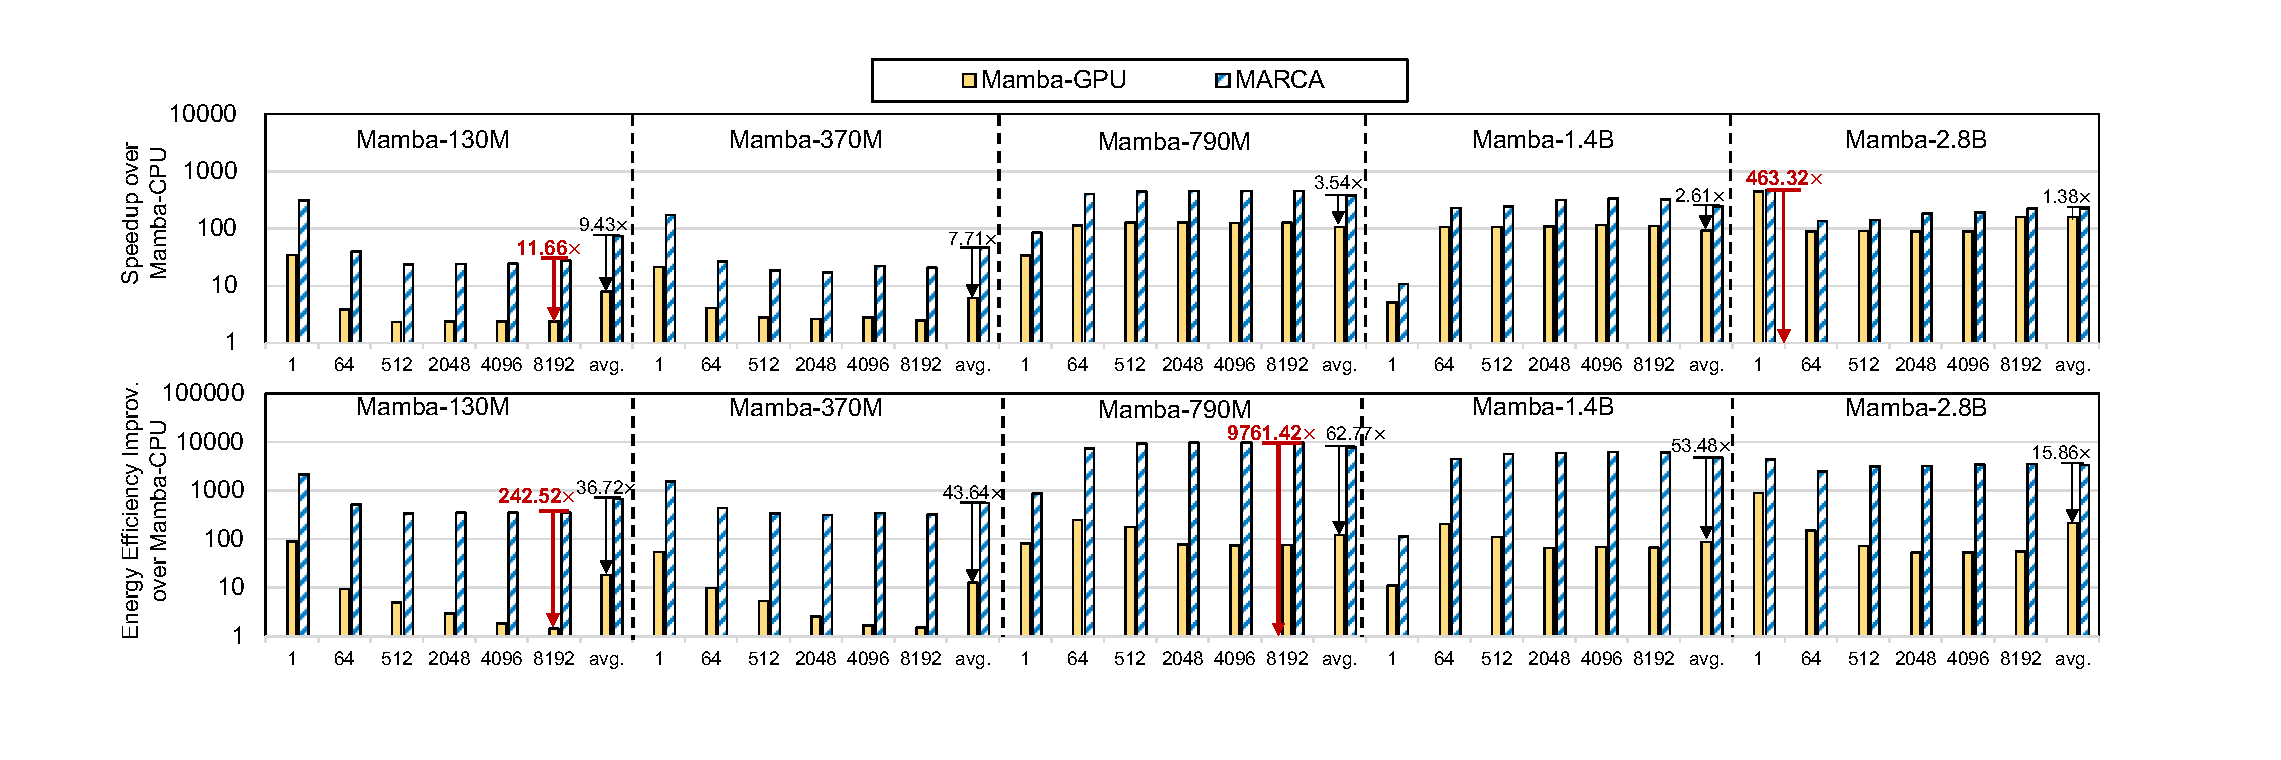
\includegraphics[width=0.99\textwidth]{figures/experiment/speedup.pdf}
%   \vspace{-10pt}
%   \caption{Comparison of speedup and energy efficiency improvement to Mamba-CPU and Mamba-GPU on Mamba models with different input sequence length.}
%   \vspace{-13pt}
%   \label{fig:speedup}
% \end{figure*}

% \subsection{Hardware Evaluations}
% We compare our work with Mamba-CPU and Mamba-GPU in terms of speedup and energy consumption,
% Finally, the area and power of our design is presented.

% % \textbf{\textit{\underline{Speedup.}}}
% \textbf{Speedup.}
% Figure~\ref{fig:speedup} top depicts that \we achieves up to 463.32$\times$/11.66$\times$ speedup and average 194.26$\times$/4.93$\times$ speedup compared with Mamba-CPU and Mamba-GPU, respectively.
% The performance improvement comes from the reconfigurable architecture, and the intra-operation and inter-operation buffer management strategy. 
% First, the reconfigurable computing unit with several reconfigurable processing element arrays accelerate the computations. 
% Second, the intra-operation input data sharing and inter-operation data sharing methods reduce large redundant data between global memory and on-chip memory.
% % Finally, the nonlinear functions are approximated and decomposed into several element-wise operations to reuse the reconfigurable computing units, which improves hardware utilization.



% % \textbf{\textit{\underline{Energy Consumption.}}}
% \textbf{Energy Efficiency.}
% As Figure~\ref{fig:speedup} bottom shows, \we improves up to 9761.42$\times$/242.52$\times$ and average 3415.55$\times$/42.49$\times$ energy efficiency compared to Mamba-CPU and Mamba-GPU, respectively. 
% We consider the energy consumption of all platforms includes the off-chip memory.

% \textbf{Power and Area.}
% The total power and area of \we are only 10.44 $W$ and 221.88 $mm^2$, respectively. 
% For the on-chip buffer, we use eDRAM to reduce both the area and energy consumption. 
% For the computation precision, we use 32-bit fixed point that is enough to maintain the accuracy of Mamba inference. 
% Table~\ref{tab:pwr_and_area} provides area and power breakdown.
% The on-chip buffer consumes most of power (>60\%) and area ($\sim$80\%) to support more memory access and data sharing for element-wise operations.
% The compute engine consume 38.67\% power and 20.57\% area to perform the linear, element-wise, exponential, and SiLU computations.
% The others are small owing to the simple implementations of normalization, and instruction fetching and decoding.

% \begin{table}[htbp]
% \small
%     \centering
%     \vspace{-10pt}
%     \caption{Layout Characteristics of \we}
%     \vspace{-12pt}
%     \begin{tabular}{cccc}
%         \toprule
%         \textbf{Component} & \textbf{Sub-module} & \textbf{Area} ($mm^2$/\%) & \textbf{Power} ($W$/\%) \\
%         \midrule
%         Inst. Processing & - & 0.45/0.20\% & 0.045/0.43\%\\
%         \midrule
%         Norm. Unit & - & 0.06/0.03\% & 0.003/0.03\%\\
%         \midrule
%         \multirow{4}{*}{Compute Engine} & RPEs & 44.87/20.22\% & 3.92/37.55\% \\
%         & Reduction Trees & 0.47/0.21\% & 0.053/0.51\% \\
%         & Control Unit & 0.32/0.14\% & 0.064/0.61\% \\
%         \cmidrule(lr){2-4}
%         & - & 45.66/20.57\% & 4.037/38.67\% \\
%         \midrule
%         On-chip Buffer & - & 175.71/79.19\% & 6.35/60.87\%\\  
%         \midrule
%         Total & - & 221.88/100\% & 10.44/100\%\\ 
%         \bottomrule
%     \end{tabular}
%     \vspace{-12pt}
%     \label{tab:pwr_and_area}
% \end{table}


% \subsection{Ablation Study}
% % We also present an ablation study to validate the superiority of our RCU over the Tensor Core-based architecture and our buffer management strategy over the no sharing (naive) strategy. 

% \textbf{Speedup of RCU over Tensor Core.}
% Figure~\ref{fig:ablation} top left shows the speedup from 1.41$\times$ to 11.95$\times$ over Tensor Core-based architecture with different sequence length in Mamba. 

% \textbf{Normalized area of RPE.}
% In Figure~\ref{fig:ablation} top right, we compare the normalized PE area overhead by supporting different nonlinear functions.
% It shows that our reusable RPE only increases 14\% area overhead.

% \textbf{Normalized memory access improvement.}
% Figure~\ref{fig:ablation} bottom reveals the normalized global memory access with out buffer management strategy. When the sequence is short, linear operations are dominant, the intra-BM reduces 73\% memory access significantly. The inter-BM reduces 49\% memory access with long sequence.

% \begin{figure}[!t]
%   \centering
%   % \vspace{-5pt}
%   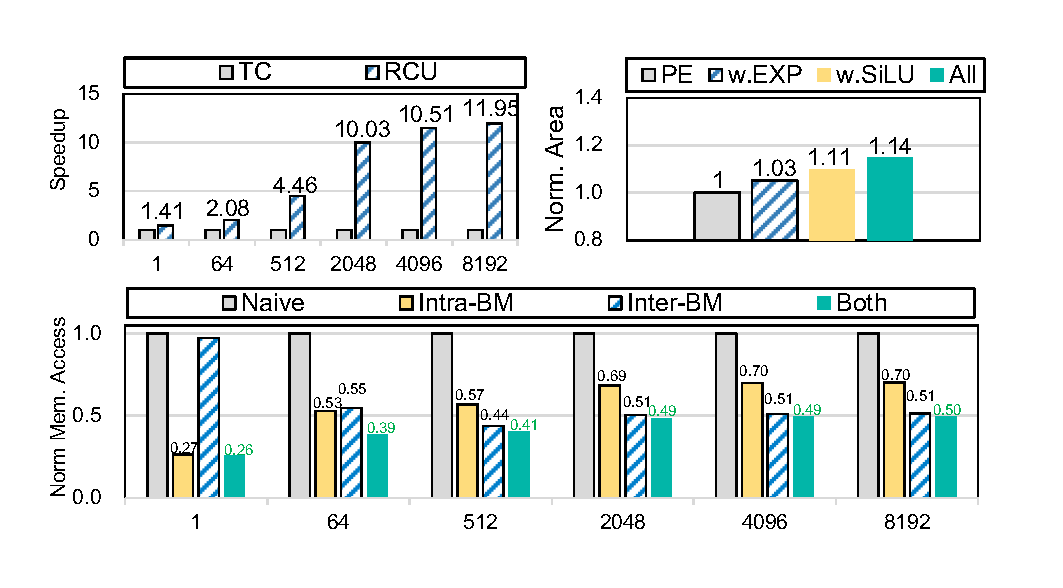
\includegraphics[width=0.47\textwidth]{figures/experiment/ablation.pdf}
%   \vspace{-15pt}
%   \caption{Ablation study: (1) Speedup of RCU over Tensor Core. (2) Normalized area of RPE. (3) Normalized memory access of intra-/inter-operation buffer management strategy.}
%   \vspace{-15pt}
%   \label{fig:ablation}
% \end{figure}

% % \begin{figure}[!t]
% %   \centering
% %   % \vspace{-10pt}
% %   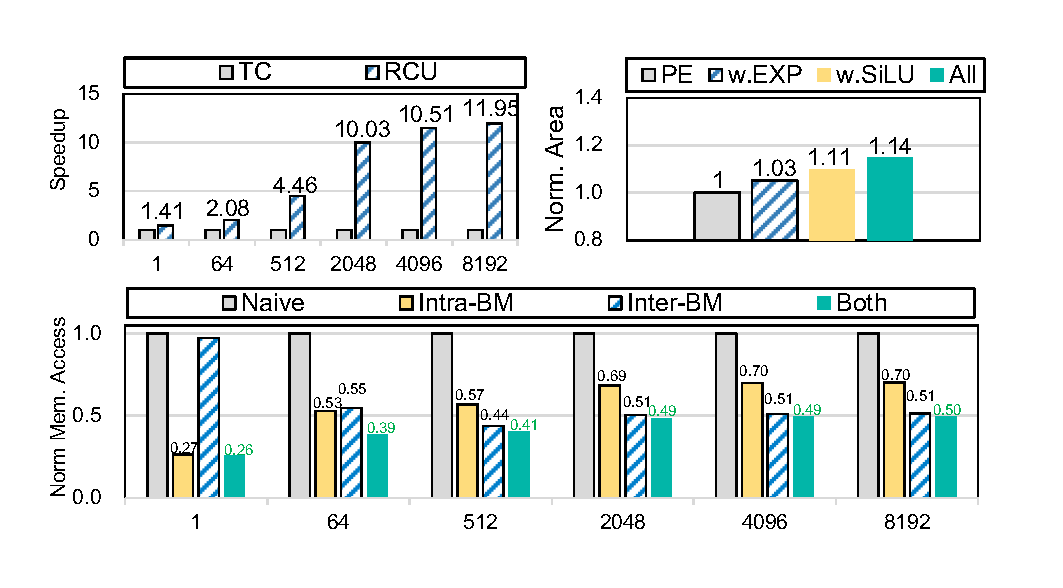
\includegraphics[width=0.48\textwidth]{figures/experiment/ablation.pdf}
% %   \vspace{-20pt}
% %   \caption{Ablation study 2: Normalized memory access of operation-wise buffer management strategy.}
% %   \vspace{-10pt}
% %   \label{fig:ablation2}
% % \end{figure}

\section{Conclusions}\label{sec:conclusion}
% Our \we is the first proposed accelerator with reconfigurable architecture specifically tailored for Mamba computations.
% We propose a reduction alternative PE array architecture to support both linear and element-wise operations. 
% Then, based on the reconfigurable PE, we decompose the nonlinear functions and reuse PE arrays reduce the area overhead.
% We also propose intra-operation and inter-operation buffer management strategy to maximize data reuse for two dominant operations.
% We conduct extensive experiments on Mamba model families with different model sizes.
% \we achieves up to 463.22$\times$/11.66$\times$ speedup and up to 9761.42$\times$/242.52$\times$ energy efficiency compared to Intel Xeon 8358P CPU and NVIDIA Tesla A100 GPU implementations, respectively. 



\section{Acknowledgments}
% This work was supported by the National Natural Science Foundation of China (No. 62104128, U21B2031), Beijing Douyin Information Service Co., Ltd.



%%
%% The next two lines define the bibliography style to be used, and
%% the bibliography file.
\bibliographystyle{ACM-Reference-Format}
\bibliography{refs1}


\end{document}
\endinput
%%
%% End of file `sample-sigplan.tex'.
